% Options for packages loaded elsewhere
\PassOptionsToPackage{unicode}{hyperref}
\PassOptionsToPackage{hyphens}{url}
%
\documentclass[
]{article}
\usepackage{lmodern}
\usepackage{amssymb,amsmath}
\usepackage{ifxetex,ifluatex}
\ifnum 0\ifxetex 1\fi\ifluatex 1\fi=0 % if pdftex
  \usepackage[T1]{fontenc}
  \usepackage[utf8]{inputenc}
  \usepackage{textcomp} % provide euro and other symbols
\else % if luatex or xetex
  \usepackage{unicode-math}
  \defaultfontfeatures{Scale=MatchLowercase}
  \defaultfontfeatures[\rmfamily]{Ligatures=TeX,Scale=1}
\fi
% Use upquote if available, for straight quotes in verbatim environments
\IfFileExists{upquote.sty}{\usepackage{upquote}}{}
\IfFileExists{microtype.sty}{% use microtype if available
  \usepackage[]{microtype}
  \UseMicrotypeSet[protrusion]{basicmath} % disable protrusion for tt fonts
}{}
\makeatletter
\@ifundefined{KOMAClassName}{% if non-KOMA class
  \IfFileExists{parskip.sty}{%
    \usepackage{parskip}
  }{% else
    \setlength{\parindent}{0pt}
    \setlength{\parskip}{6pt plus 2pt minus 1pt}}
}{% if KOMA class
  \KOMAoptions{parskip=half}}
\makeatother
\usepackage{xcolor}
\IfFileExists{xurl.sty}{\usepackage{xurl}}{} % add URL line breaks if available
\IfFileExists{bookmark.sty}{\usepackage{bookmark}}{\usepackage{hyperref}}
\hypersetup{
  pdftitle={Step1 Team Project Multivariate Analysis},
  pdfauthor={Adrian White, Cesar Conejo, Xavier Bryant},
  hidelinks,
  pdfcreator={LaTeX via pandoc}}
\urlstyle{same} % disable monospaced font for URLs
\usepackage[margin=1in]{geometry}
\usepackage{longtable,booktabs}
% Correct order of tables after \paragraph or \subparagraph
\usepackage{etoolbox}
\makeatletter
\patchcmd\longtable{\par}{\if@noskipsec\mbox{}\fi\par}{}{}
\makeatother
% Allow footnotes in longtable head/foot
\IfFileExists{footnotehyper.sty}{\usepackage{footnotehyper}}{\usepackage{footnote}}
\makesavenoteenv{longtable}
\usepackage{graphicx}
\makeatletter
\def\maxwidth{\ifdim\Gin@nat@width>\linewidth\linewidth\else\Gin@nat@width\fi}
\def\maxheight{\ifdim\Gin@nat@height>\textheight\textheight\else\Gin@nat@height\fi}
\makeatother
% Scale images if necessary, so that they will not overflow the page
% margins by default, and it is still possible to overwrite the defaults
% using explicit options in \includegraphics[width, height, ...]{}
\setkeys{Gin}{width=\maxwidth,height=\maxheight,keepaspectratio}
% Set default figure placement to htbp
\makeatletter
\def\fps@figure{htbp}
\makeatother
\setlength{\emergencystretch}{3em} % prevent overfull lines
\providecommand{\tightlist}{%
  \setlength{\itemsep}{0pt}\setlength{\parskip}{0pt}}
\setcounter{secnumdepth}{-\maxdimen} % remove section numbering

\title{Step1 Team Project Multivariate Analysis}
\author{Adrian White, Cesar Conejo, Xavier Bryant}
\date{12/6/2020}

\begin{document}
\maketitle

\hypertarget{introduction-data-set}{%
\subsection{Introduction data set}\label{introduction-data-set}}

We have selected the
\href{https://hbiostat.org/data/repo/crash2.html}{CRASH-2} data set
provided by the Bank of Injury and Emergency Research Data from the UK.
It describes the outcome of a randomized controlled trial and economic
valuation of the effects of tranexamic acid on death, vascular occlusive
events, and transfusion requirement in bleeding trauma patients.
Tranexamic acid reduces bleeding in trauma patients undergoing surgery
but is an expensive treatment option. The trial's objective was to
assess the effects and cost-effectiveness of an early administration of
this medication.

Participants of the study were adults with, or at risk of, significant
bleeding within 8 hours of injury. Sample randomization was determined
by the allocation of an eight-digit sequence randomly generated by a
computer. Patients and staff were masked to the treatment allocation of
the tranexamic acid.Patients and staff were masked to the treatment
allocation of the tranexamic acid. However, the data set reflects some
information in case of the decease of patients. As a result, we create a
categorical variable called \emph{death} with the final states 1 in case
of passing and 0 if the patient survives.

We have adjusted the original data set to remove some variables that
were not relevant to our investigation. We have removed variables
regarding the exact surgical procedures administered to patients,
various IDs, and details on the patient outcome. We removed the health
outcome columns because of complications regarding missing data, where
the boolean structure of the columns relating to specific outcomes, like
stroke or pulmonary embolism, left a large number of cases with missing
values. Instead, we added a boolean variable for a general outcome of
survival to assess the efficacy of the procedure, rather than looking at
particular health outcomes in post-surgery for living patients.

We will be using variables regarding the sex, age, and injury of the
patient as well as certain biometrics, like blood pressure, respiratory
and heart rates, details on surgical blood transfusion, and a boolean
variable on the survival of the patient. Our selection provides us with
a balance of continuous and categorical variables, many of which are
boolean, with minimal complications due to missing data. In summary, the
data set consists of \(n = 9497\) observations, with 11 columns, which
\(p = 8\) are quantitative and 3 are qualitative.

Moreover, the normal ranges of the biometric measurements are also
added, in order to have a point of comparison with the observations
present in the data set and in this way determine if they are abnormal
with respect to the normal metrics.

\newpage

\hypertarget{summary-variables-in-the-data-set}{%
\subsubsection{Summary variables in the data
set}\label{summary-variables-in-the-data-set}}

The variables in this dataset are the following:

\begin{enumerate}
\def\labelenumi{\arabic{enumi}.}
\item
  sex: (Boolean) The sex of the patient (Male/Female)
\item
  age : (Numerical) Age of the patient(Years)
\item
  injurytime: (Numerical) Hours since injury (Hours)
\item
  injurytype: (Categorical) Type of injury \{Blunt, Penetrating, Blunt
  and Penetrating\}
\item
  sbp: (Numerical) Systolic Blood Pressure (mmHg). Normal range for
  adults at rest: less 120 mmHg.
\item
  rr: (Numerical) Respiratory Rate (breaths per minute). Normal range
  for adults at rest: 12 - 20 breaths per minute.
\item
  cc: (Numerical) Central Capillary Refill Time (seconds). Normal range
  for adults at rest. Less than 3 seconds.
\item
  hr: (Numerical) Heart Rate (beats per minute). Normal range for adults
  at rest: 60 - 100 bpm.
\item
  ndaysicu: (Numerical) Number of days in ICU (days)
\item
  ncell: (Numerical) Number of Units of Red Call Products Transfused.
\item
  death: (Boolean) Indicator if the patient survived after the procedure
\end{enumerate}

A summary of the data type is the following:

\begin{longtable}[]{@{}lll@{}}
\toprule
variable & type\_variable & sub\_type\_variable\tabularnewline
\midrule
\endhead
sex & Qualitative & Nominal\tabularnewline
age & Quantitative & Continuous\tabularnewline
injurytime & Quantitative & Continuous\tabularnewline
injurytype & Qualitative & Nominal\tabularnewline
sbp & Quantitative & Continuous\tabularnewline
rr & Quantitative & Continuous\tabularnewline
cc & Quantitative & Continuous\tabularnewline
hr & Quantitative & Continuous\tabularnewline
ndaysicu & Quantitative & Discrete\tabularnewline
ncell & Quantitative & Continuous\tabularnewline
death & Qualitative & Nominal\tabularnewline
\bottomrule
\end{longtable}

A review of the structure of the data set is the following:

\begin{verbatim}
## 'data.frame':    9497 obs. of  11 variables:
##  $ sex       : Factor w/ 2 levels "male","female": 1 1 1 1 1 1 1 1 1 2 ...
##  $ age       : int  50 30 40 19 27 16 29 41 56 37 ...
##  $ injurytime: num  1 1 2 3 0.5 1 1 0.5 0.5 8 ...
##  $ injurytype: Factor w/ 3 levels "blunt","penetrating",..: 1 1 2 2 2 2 1 2 1 2 ...
##  $ sbp       : int  75 70 60 90 90 90 116 120 60 104 ...
##  $ rr        : int  28 26 20 30 26 28 15 15 9 23 ...
##  $ cc        : int  5 6 5 5 5 2 3 3 3 5 ...
##  $ hr        : int  120 130 120 90 96 118 118 70 100 92 ...
##  $ ndaysicu  : num  0 6 2 9 7 0 7 7 23 2 ...
##  $ ncell     : num  1 2 4 2 1 1 16 8 4 4 ...
##  $ death     : Factor w/ 2 levels "0","1": 2 1 2 2 1 1 1 1 1 1 ...
\end{verbatim}

\newpage

A summary of the values in the data set are:

\begin{verbatim}
##      sex            age          injurytime                     injurytype  
##  male  :7906   Min.   :14.00   Min.   : 0.100   blunt                :5211  
##  female:1591   1st Qu.:24.00   1st Qu.: 1.000   penetrating          :2937  
##                Median :31.00   Median : 3.000   blunt and penetrating:1349  
##                Mean   :34.66   Mean   : 3.094                               
##                3rd Qu.:43.00   3rd Qu.: 4.500                               
##                Max.   :96.00   Max.   :48.000                               
##       sbp               rr              cc               hr       
##  Min.   :  4.00   Min.   : 2.00   Min.   : 1.000   Min.   :  3.0  
##  1st Qu.: 80.00   1st Qu.:20.00   1st Qu.: 2.000   1st Qu.: 96.0  
##  Median : 90.00   Median :22.00   Median : 3.000   Median :110.0  
##  Mean   : 93.13   Mean   :23.46   Mean   : 3.438   Mean   :108.1  
##  3rd Qu.:104.00   3rd Qu.:28.00   3rd Qu.: 4.000   3rd Qu.:120.0  
##  Max.   :225.00   Max.   :91.00   Max.   :20.000   Max.   :220.0  
##     ndaysicu          ncell        death   
##  Min.   : 0.000   Min.   : 0.000   0:7672  
##  1st Qu.: 0.000   1st Qu.: 2.000   1:1825  
##  Median : 1.000   Median : 3.000           
##  Mean   : 4.137   Mean   : 3.912           
##  3rd Qu.: 5.000   3rd Qu.: 5.000           
##  Max.   :58.000   Max.   :60.000
\end{verbatim}

Finally, the list of different values by column is the following:

\begin{longtable}[]{@{}ccccccccccc@{}}
\caption{Count of distinct values of each variable}\tabularnewline
\toprule
sex & age & injurytime & injurytype & sbp & rr & cc & hr & ndaysicu &
ncell & death\tabularnewline
\midrule
\endfirsthead
\toprule
sex & age & injurytime & injurytype & sbp & rr & cc & hr & ndaysicu &
ncell & death\tabularnewline
\midrule
\endhead
2 & 81 & 78 & 3 & 153 & 58 & 16 & 154 & 47 & 47 & 2\tabularnewline
\bottomrule
\end{longtable}

\newpage

\hypertarget{visual-analysis}{%
\subsection{Visual Analysis}\label{visual-analysis}}

\hypertarget{univariate-analysis}{%
\subsubsection{Univariate Analysis}\label{univariate-analysis}}

First, we will review the distribution of the variables involved in the
data set.

In the case of \emph{age}, the Figure \ref{fig:age} reflects how this
variable appears to be largely weighted to the left, with lower ages
featuring more frequently than those that are greater, possibly
reflecting that younger people often take more risk and work higher
at-risk occupations, raising their chance of experiencing trauma
involving bleeding.

\begin{figure}
\centering
\includegraphics{Step1_Project_files/figure-latex/age-1.pdf}
\caption{Distribution of age variable\label{fig:age}}
\end{figure}

Figure \ref{fig:injurytime} below shows the distribution of the variable
for injury time (\emph{injurytime}) We can see how this variable is
highly skewed to the left with almost all values falling below ten
minutes since the injury was experienced. This is likely due to the
fact, that in cases of serious injury, victims are brought to the
hospital quite quickly as is the case for this data set on trauma. We
apply a \emph{log} transformation to this variable
\texttt{log\_injurytime\ =\ log(injurytime\ +\ 1)}, similarly to many
other variables we have, because of the weight of the variables to the
left of the distribution, in order to make a more normalized
distribution. After the \emph{log} transformation, we can see that two
observations remain quite distinct and far to the right, with a value of
four. They appear as potential outliers to the distribution, as they
have almost 4 times the median value.

\begin{figure}
\centering
\includegraphics{Step1_Project_files/figure-latex/injurytime-1.pdf}
\caption{Distribution of injurytime variable and log of
injurytime\label{fig:injurytime}}
\end{figure}

For \emph{sbp} (systolic blood pressure), the distribution is a fairly
centrally balanced distribution around 90 mmHg. Most observations around
the mean and then a reasonably tight distribution of those who differ,
making a distribution that is fairly Gaussian by nature. Furthermore,
most people are fairly young in the sample and therefore would have
rates, at a healthy level, that deviant less from the norm. The
distribution is shown below in Figure \ref{fig:sbp}.

\begin{figure}
\centering
\includegraphics{Step1_Project_files/figure-latex/sbp-1.pdf}
\caption{Distribution of sbp (Systolic Blood Pressure)\label{fig:sbp}}
\end{figure}

\newpage

\emph{Rr} (Respiratory Rate) appears, similar to sbp, to resemble a
moderately balanced distribution around 22 respirations per minute,
although \emph{rr} is weighted more to the left. The distribution of
this variable is shown in Figure \ref{fig:rr}. Taking a \emph{log}
transformation \texttt{log\_rr\ =\ log(rr)}, we have the new
distribution below as part of Figure \ref{fig:rr}. After the log
transformation, the distribution remains quite spread out with a number
of values beyond the whiskers of the box plot. The \emph{log}
transformation, in this case, has not significantly changed the shape of
the distribution, it does not shift much more towards a normal
distribution after the \emph{log} transformation.

\begin{figure}
\centering
\includegraphics{Step1_Project_files/figure-latex/rr-1.pdf}
\caption{Distribution of rr (Respiratory Rate) and logrr\label{fig:rr}}
\end{figure}

In the case of \emph{hr} (Heart rate), Figure \ref{fig:hr} has a
distribution that seems fairly balanced at around 110, similar to the
variables above, like \emph{sbp} and \emph{rr}. However, many values
remain outside the whiskers and the IQR is quite tight, showing most
people fall within a tight range but there is a number of people who
have irregular rates on either side.

\begin{figure}
\centering
\includegraphics{Step1_Project_files/figure-latex/hr-1.pdf}
\caption{Distribution of hh (Heart Rate)\label{fig:hr}}
\end{figure}

For \emph{cc} (Central capillary refill time in seconds) has 75\% of the
observations below roughly 4 as we can appreciate in Figure
\ref{fig:cc}. However, the distribution is right-skewed. As a result, we
apply a \emph{log} transformation \texttt{log\_cc\ =\ log(cc)} that is
given in the below part of Figure \ref{fig:cc}. The log has made the
distribution more normal and was quite successful in this case. There
remains a number of observations to the far right of the distribution,
which could be possible outliers as they represent values approximately
three times the median.

\begin{figure}
\centering
\includegraphics{Step1_Project_files/figure-latex/cc-1.pdf}
\caption{Distribution of cc (Central capillary) and log
transformation\label{fig:cc}}
\end{figure}

The following Figure \ref{fig:ndaysicu} shows the distribution of the
\emph{ndaysicu:} variable. In this case, the distribution is heavily
weighted to the left and right-skewed. Most patients it seems, with
trauma injuries at high risk of bleeding, do not often need to remain in
the hospital for long. The transformed distribution
\texttt{log\_ndaysicu\ =\ log(ndaysicu\ +\ 1)} is given in the below
part of Figure \ref{fig:ndaysicu}. After the \emph{log} transformation,
this distribution doesn't appear much more Gaussian in nature. The
values are still heavily weighted on the left. No values appear outside
the whiskers, however, therefore this leads us to believe that there is
not much likelihood of outliers in this distribution.

\begin{figure}
\centering
\includegraphics{Step1_Project_files/figure-latex/ndaysicu-1.pdf}
\caption{Distribution of ndaysicu and log
transformation\label{fig:ndaysicu}}
\end{figure}

Finally, the \emph{ncell} distribution is weighted to the left with a
median of 3 as we can see in Figure \ref{fig:ncell}. The conclusion of
this is that many patients only need a small number of or zero units of
red cell products transfused. Due to this variable being highly weighted
to the left, we apply the \emph{log} transformation
\texttt{log\_ncell\ =\ log(ncell\ +\ 1)}. After the transformation, the
variables visually appears to be more Gaussian, but a large number of
values remain outside the whiskers on the right of the distribution.
None, however, appear to be distinct enough from the others to be
outliers.

\begin{figure}
\centering
\includegraphics{Step1_Project_files/figure-latex/ncell-1.pdf}
\caption{Distribution of ncell\label{fig:ncell}}
\end{figure}

Our primary categorical variable will be the distributions of
\emph{death}, where 0 represents people who survive and 1 for those who
do not survive. Figure \ref{fig:deaths}, shows that approximately for
each death, 4 people survive. In the context of this problem, if we have
an unbalanced proportion of people that survive, it can be considered as
a sign that most people survive trauma injuries in the data set and that
with the administration of the drug, most people survive. Although, this
is not necessarily due to the treatment with the drug as both the
control and treatment sample are contained in this data set, and were
not separated (due to the absence of the treatment variable).

\begin{figure}
\centering
\includegraphics{Step1_Project_files/figure-latex/deaths-1.pdf}
\caption{Distribution of deaths\label{fig:deaths}}
\end{figure}

\newpage

\hypertarget{univariate-analysis-by-death---survival-patients}{%
\subsubsection{Univariate Analysis by death - survival
patients}\label{univariate-analysis-by-death---survival-patients}}

Our next step is to study some relations of the quantitative variables
in terms of our central categorical variable \emph{death}.

Figure \ref{fig:agedeath}, shows us that those who survive (0) are on
average younger than those who do not survive, which is logical, as
younger people likely fair better in trauma accidents where there is a
risk of significant bleeding (which this trail assesses). Aside from the
median being slightly smaller than for those who survive, the
distributions are fairly similar with a skew to the right. Participants
in this trial are on average are quite young, roughly 34.7, which could
be due to sampling, but also because younger people are more likely to
suffer from trauma accidents due to having jobs with an increased
propensity of injury and also more generally for risk-taking behavior.

\begin{figure}
\centering
\includegraphics{Step1_Project_files/figure-latex/agedeath-1.pdf}
\caption{Distribution of Age in terms of death\label{fig:agedeath}}
\end{figure}

Figure \ref{fig:loginjurytimedeath} showing \emph{log injury time}
demonstrates that those who survive (1) have longer relative injury time
on average. The IQR for those who survive is also wider as well as the
whiskers. However, there are still values of longer injury times for
those who do survive, however they appear less frequently. This is
slightly counterintuitive as we would expect those who took longer to
get to the hospital or those who have been suffering longer, would be at
a higher risk of \emph{death}. However, it's possible that these people
have less serious injuries, and have less risk of dying, and are then
rushed to hospital with less urgency, having a long injury time.

\begin{figure}
\centering
\includegraphics{Step1_Project_files/figure-latex/loginjurytimedeath-1.pdf}
\caption{Distribution of the log injurytime in terms of
death\label{fig:loginjurytimedeath}}
\end{figure}

Figure \ref{fig:sbpdeath} showing \emph{sbp} (systolic blood pressure)
against \emph{death}, shows that those who survive (O), have
distribution slightly to the right of that of the those who do not
survive. This could be logical as those who survive have a higher blood
pressure after the accident than those who eventually do not because
their bodies are less weakened by the trauma.

\begin{figure}
\centering
\includegraphics{Step1_Project_files/figure-latex/sbpdeath-1.pdf}
\caption{Distribution of sbp (Systolic Blood Pressure) in terms of
death\label{fig:sbpdeath}}
\end{figure}

\newpage

Figure \ref{fig:logrrdeath} compares \emph{log respiratory rate} (rr)
with those who do not survive (1) have a slightly higher mean than those
who survive (1). This seems to lead us to believe, that those who do not
survive, more often have a higher than average respiratory rate.

\begin{figure}
\centering
\includegraphics{Step1_Project_files/figure-latex/logrrdeath-1.pdf}
\caption{Distribution of log transformation of rr (Respiratory Rate) in
terms of death\label{fig:logrrdeath}}
\end{figure}

Figure \ref{fig:hrdeath}, similar to \emph{log respiratory rate}, the
median of the distribution of \emph{log heart rate} for those who do not
survive (1) is slightly higher than those who survive (0).

\begin{figure}
\centering
\includegraphics{Step1_Project_files/figure-latex/hrdeath-1.pdf}
\caption{Distribution of hh (hearth Rate) in terms of
death\label{fig:hrdeath}}
\end{figure}

\newpage

Figure \ref{fig:logccdeath}, also resembling \emph{log heart rate (hr)}
and \emph{log respiratory rate (rr)}, \emph{log central capillary (cc)}
(central capillary refill time in seconds) has a distribution further to
the right, even more extreme than \emph{hr} and \emph{rr}, which could
show that \emph{cc} increases like \emph{hr} and \emph{rr} on average
for people who will not survive. We also remain to see a limited number
of observations to the extreme right, which could be outliers.

\begin{figure}
\centering
\includegraphics{Step1_Project_files/figure-latex/logccdeath-1.pdf}
\caption{Distribution of log transformation of cc (Central capillary) in
terms of death\label{fig:logccdeath}}
\end{figure}

Figure \ref{fig:logndaysicudeath} shows that days in the ICU
(\emph{ndaysicu}), has a very similar distribution with an identical
median, likely due to the fact that most people who suffer from trauma
injuries only spend a very limited relative amount of time in the ICU.
We see that, for those who survive (0), the 75\% quartile is slightly
larger, and when reviewing the histogram, more observations are on the
further right end of the spectrum (more relative days in hospital). This
possibly indicates to us that those who are more likely to survive are
kept in the ICU for longer to heal in some cases.

\begin{figure}
\centering
\includegraphics{Step1_Project_files/figure-latex/logndaysicudeath-1.pdf}
\caption{Distribution of log ndaysicu in terms of
death\label{fig:logndaysicudeath}}
\end{figure}

\newpage

Figure \ref{fig:logncelldeath} shows the \emph{log} value of red blood
cells transfused (\emph{ncell}) accounting for \emph{death}. Those who
do not survive (1), have a broader distribution with the 75\% quartile
being larger, possibly indicating that for those who will not survive,
more blood cells are transfused for more grave injuries that are less
survivable.

\begin{figure}
\centering
\includegraphics{Step1_Project_files/figure-latex/logncelldeath-1.pdf}
\caption{Distribution of log ncell in terms of
death\label{fig:logncelldeath}}
\end{figure}

Finally, in the scatter plot in Figure 18 we cannot see any significant
relationships but the variables, while accounting for Death. There does
not seem to be any visual relationship between any of the variables that
are outstanding.

Furthermore, the PCP plot in Figure 19, generally matches with our
observations about the scatter plots. Those who survive and do not,
follow the same visual pattern. For \emph{log\_cc}, \emph{hr}, and
\emph{log\_ndaysicu}, those who survive appear to have values that are
more broadly dispersed, but this could be due to the fact those who
survive represent a majority of the sample size, making the visual
depiction incorrect. Although comparing with the histograms and box
plots, \emph{log\_cc}, \emph{hr}, and \emph{log\_ndaysicu} does appear
to have more dispersed distributions and wider IQRs.

\newpage

\begin{figure}
\centering
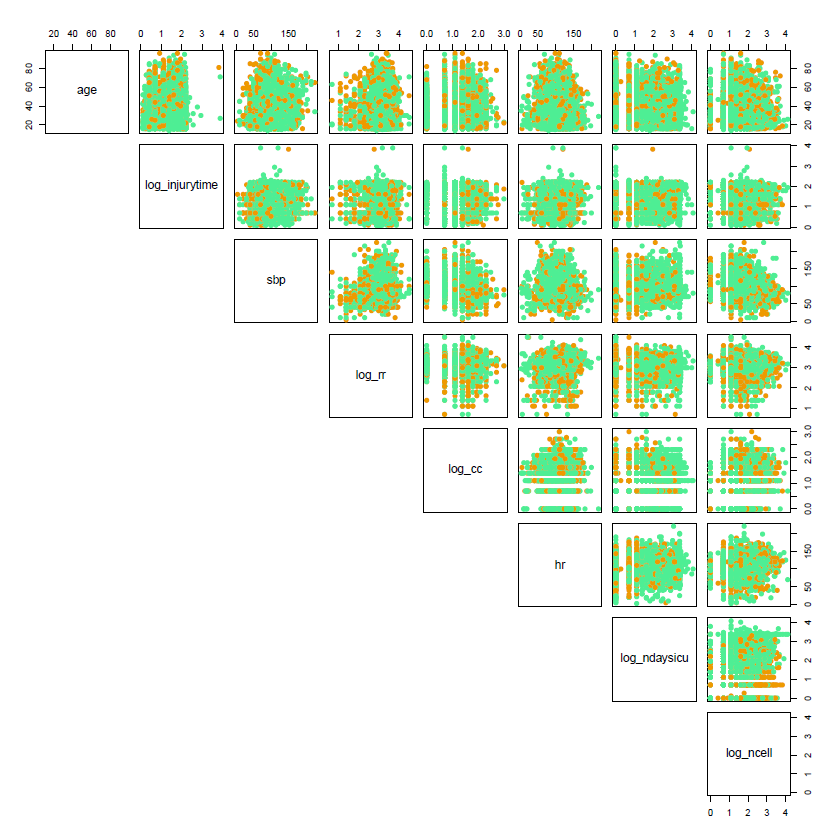
\includegraphics{../figure_output/pairs_death.png}
\caption{Scatter plot of all quantitiative variables}
\end{figure}

\newpage

\begin{figure}
\centering
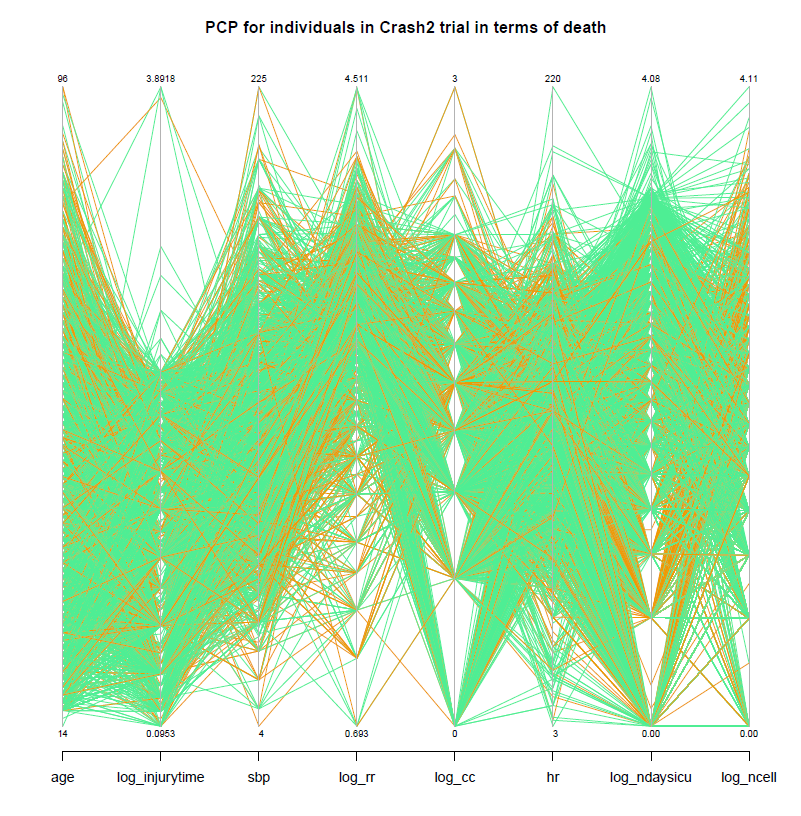
\includegraphics{../figure_output/pcp_death.png}
\caption{PCP plot of all quantitiative variables}
\end{figure}

\newpage

The Andrews' plot in Figure 20, matches our previous analysis in Figure
18 and 19, that variables share similar distributions and relationships
when accounting for \emph{death}, as the Andrew Plot does not show any
dramatic differences between the two groups.

\begin{figure}
\centering
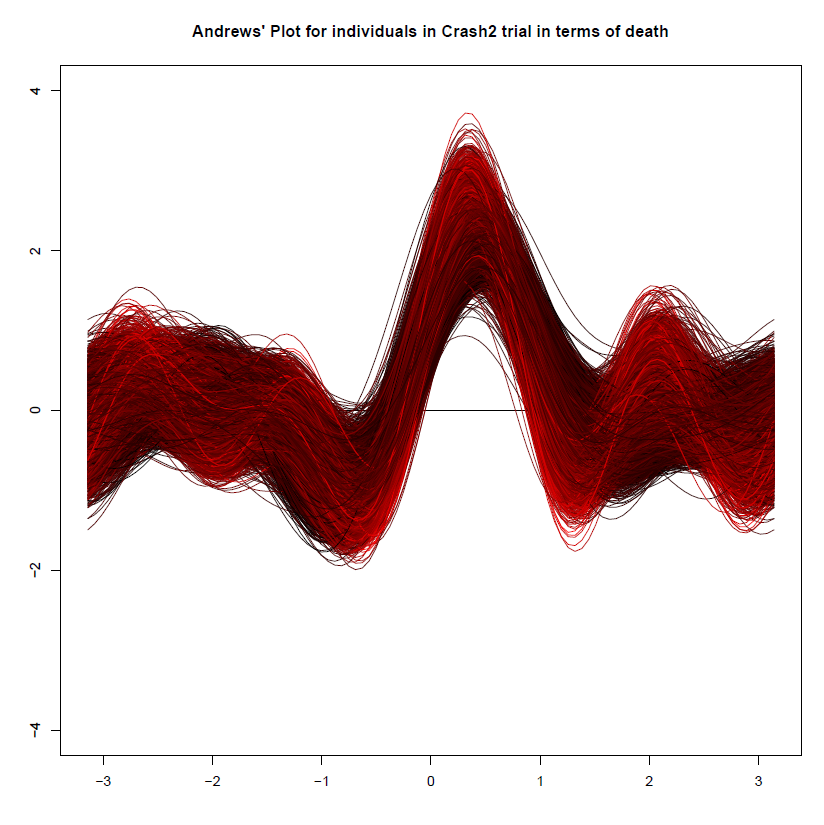
\includegraphics{../figure_output/andrew_death.png}
\caption{Andrews' plot of all quantitiative variables}
\end{figure}

In conclusion, we see that when accounting for different categorical
variables and \emph{death}, the relationships between our quantitative
variables do not change significantly overall, looking at the scatter
plots and other visuals. There doesn't appear to be any collinearity,
whether \emph{death} is accounted for or not. We can see some minor
changes in distributions and means when dividing the distribution for
those who do not and do survive, however, there is nothing too drastic.
The IQRs for all our variables overlap, for example. The medians are
even the same for \emph{log\_ncell} and \emph{log\_ndaysicu}. The
variable with the largest difference appears to be, \emph{log\_cc} where
the median for those who survive is at the 25\% quartile of those who do
not survive. For \emph{sbp}, the median for those who do not survive is
similar to the 25\% quartile of those who survive.

In the next section, we will make inferences using sample estimators of
mean, covariance, and correlation.

\newpage

\hypertarget{sample-estimators}{%
\subsection{Sample Estimators}\label{sample-estimators}}

\hypertarget{sample-mean}{%
\subsubsection{Sample mean}\label{sample-mean}}

Below is the sample mean vector for all the variables in our analysis,
without controlling for \emph{death}.

\begin{longtable}[]{@{}cccccccc@{}}
\caption{Sample mean}\tabularnewline
\toprule
age & sbp & hr & log\_injurytime & log\_rr & log\_cc & log\_ndaysicu &
log\_ncell\tabularnewline
\midrule
\endfirsthead
\toprule
age & sbp & hr & log\_injurytime & log\_rr & log\_cc & log\_ndaysicu &
log\_ncell\tabularnewline
\midrule
\endhead
34.66474 & 93.12909 & 108.0621 & 1.26759 & 3.106722 & 1.116876 &
0.9976935 & 1.394665\tabularnewline
\bottomrule
\end{longtable}

This table shows the mean while setting \emph{death} to 1, or for those
who do not survive.

\begin{longtable}[]{@{}cccccccc@{}}
\caption{Sample mean: Do not survive}\tabularnewline
\toprule
age & sbp & hr & log\_injurytime & log\_rr & log\_cc & log\_ndaysicu &
log\_ncell\tabularnewline
\midrule
\endfirsthead
\toprule
age & sbp & hr & log\_injurytime & log\_rr & log\_cc & log\_ndaysicu &
log\_ncell\tabularnewline
\midrule
\endhead
37.82849 & 87.33808 & 111.4559 & 1.240578 & 3.110272 & 1.232432 &
0.9390286 & 1.524647\tabularnewline
\bottomrule
\end{longtable}

Now provided is the sample mean for the variables when the patient
survives, or when \emph{death} = 0.

\begin{longtable}[]{@{}cccccccc@{}}
\caption{Sample mean: Survive}\tabularnewline
\toprule
age & sbp & hr & log\_injurytime & log\_rr & log\_cc & log\_ndaysicu &
log\_ncell\tabularnewline
\midrule
\endfirsthead
\toprule
age & sbp & hr & log\_injurytime & log\_rr & log\_cc & log\_ndaysicu &
log\_ncell\tabularnewline
\midrule
\endhead
33.91215 & 94.50665 & 107.2548 & 1.274015 & 3.105878 & 1.089387 &
1.011649 & 1.363745\tabularnewline
\bottomrule
\end{longtable}

Although touched upon above in our analysis of the box plots and
histograms, comparing the means when controlling for \emph{death},
overall, we do see some differences in the variables. The means of those
who survive are more similar to the overall sample mean as those who
survive represent more of the sample population. In terms of the
difference between means we see that \emph{age} is slightly higher for
those who do not survive, which is logical, as those who are younger
will likely be of better overall health and survive a trauma.\emph{Hr},
\emph{log\_rr}, \emph{log\_cc} and \emph{log\_ncell} are all higher, and
\emph{sbp} lower, for those who do not survive which could be various
responses related to the bodies response to more serious injury and it's
medical treatment (more blood given, for example).
\emph{Log\_injurytime} and \emph{log\_ndaysicu} are higher for those who
survive, possibly as those who have less serious injuries have a higher
likelihood to survive and take longer to get to a hospital. For similar
reasons, \emph{log\_ndaysicu} could be longer for those who survive as
those with more serious injuries were not able to survive for long, but
those who could survive stayed longer in the ICU.

\newpage

\hypertarget{sample-covariance}{%
\subsubsection{Sample covariance}\label{sample-covariance}}

Below are the sample covariance matrices for the general sample, and
then for those who do not survive (1) and those who survive (0). The
diagonal is the variances of the variables and the other values outside
of the diagonals identify the covariances for the corresponding
variables of the intersection of the respective row and column.

\begin{longtable}[]{@{}lcccccccc@{}}
\caption{Sample covariance matrix}\tabularnewline
\toprule
\begin{minipage}[b]{0.09\columnwidth}\raggedright
\strut
\end{minipage} & \begin{minipage}[b]{0.08\columnwidth}\centering
age\strut
\end{minipage} & \begin{minipage}[b]{0.09\columnwidth}\centering
sbp\strut
\end{minipage} & \begin{minipage}[b]{0.09\columnwidth}\centering
hr\strut
\end{minipage} & \begin{minipage}[b]{0.10\columnwidth}\centering
log\_injurytime\strut
\end{minipage} & \begin{minipage}[b]{0.07\columnwidth}\centering
log\_rr\strut
\end{minipage} & \begin{minipage}[b]{0.07\columnwidth}\centering
log\_cc\strut
\end{minipage} & \begin{minipage}[b]{0.09\columnwidth}\centering
log\_ndaysicu\strut
\end{minipage} & \begin{minipage}[b]{0.07\columnwidth}\centering
log\_ncell\strut
\end{minipage}\tabularnewline
\midrule
\endfirsthead
\toprule
\begin{minipage}[b]{0.09\columnwidth}\raggedright
\strut
\end{minipage} & \begin{minipage}[b]{0.08\columnwidth}\centering
age\strut
\end{minipage} & \begin{minipage}[b]{0.09\columnwidth}\centering
sbp\strut
\end{minipage} & \begin{minipage}[b]{0.09\columnwidth}\centering
hr\strut
\end{minipage} & \begin{minipage}[b]{0.10\columnwidth}\centering
log\_injurytime\strut
\end{minipage} & \begin{minipage}[b]{0.07\columnwidth}\centering
log\_rr\strut
\end{minipage} & \begin{minipage}[b]{0.07\columnwidth}\centering
log\_cc\strut
\end{minipage} & \begin{minipage}[b]{0.09\columnwidth}\centering
log\_ndaysicu\strut
\end{minipage} & \begin{minipage}[b]{0.07\columnwidth}\centering
log\_ncell\strut
\end{minipage}\tabularnewline
\midrule
\endhead
\begin{minipage}[t]{0.09\columnwidth}\raggedright
age\strut
\end{minipage} & \begin{minipage}[t]{0.08\columnwidth}\centering
201.8020767\strut
\end{minipage} & \begin{minipage}[t]{0.09\columnwidth}\centering
5.6687061\strut
\end{minipage} & \begin{minipage}[t]{0.09\columnwidth}\centering
-26.9775900\strut
\end{minipage} & \begin{minipage}[t]{0.10\columnwidth}\centering
0.5843356\strut
\end{minipage} & \begin{minipage}[t]{0.07\columnwidth}\centering
0.0754442\strut
\end{minipage} & \begin{minipage}[t]{0.07\columnwidth}\centering
0.3511496\strut
\end{minipage} & \begin{minipage}[t]{0.09\columnwidth}\centering
1.1379316\strut
\end{minipage} & \begin{minipage}[t]{0.07\columnwidth}\centering
0.1173186\strut
\end{minipage}\tabularnewline
\begin{minipage}[t]{0.09\columnwidth}\raggedright
sbp\strut
\end{minipage} & \begin{minipage}[t]{0.08\columnwidth}\centering
5.6687061\strut
\end{minipage} & \begin{minipage}[t]{0.09\columnwidth}\centering
604.1019094\strut
\end{minipage} & \begin{minipage}[t]{0.09\columnwidth}\centering
-117.2846636\strut
\end{minipage} & \begin{minipage}[t]{0.10\columnwidth}\centering
1.8258493\strut
\end{minipage} & \begin{minipage}[t]{0.07\columnwidth}\centering
-0.3695028\strut
\end{minipage} & \begin{minipage}[t]{0.07\columnwidth}\centering
-2.8828312\strut
\end{minipage} & \begin{minipage}[t]{0.09\columnwidth}\centering
1.6117323\strut
\end{minipage} & \begin{minipage}[t]{0.07\columnwidth}\centering
-1.9082923\strut
\end{minipage}\tabularnewline
\begin{minipage}[t]{0.09\columnwidth}\raggedright
hr\strut
\end{minipage} & \begin{minipage}[t]{0.08\columnwidth}\centering
-26.9775900\strut
\end{minipage} & \begin{minipage}[t]{0.09\columnwidth}\centering
-117.2846636\strut
\end{minipage} & \begin{minipage}[t]{0.09\columnwidth}\centering
459.8457610\strut
\end{minipage} & \begin{minipage}[t]{0.10\columnwidth}\centering
-0.0753408\strut
\end{minipage} & \begin{minipage}[t]{0.07\columnwidth}\centering
1.3004116\strut
\end{minipage} & \begin{minipage}[t]{0.07\columnwidth}\centering
0.8685547\strut
\end{minipage} & \begin{minipage}[t]{0.09\columnwidth}\centering
0.9063157\strut
\end{minipage} & \begin{minipage}[t]{0.07\columnwidth}\centering
1.4739129\strut
\end{minipage}\tabularnewline
\begin{minipage}[t]{0.09\columnwidth}\raggedright
log\_injurytime\strut
\end{minipage} & \begin{minipage}[t]{0.08\columnwidth}\centering
0.5843356\strut
\end{minipage} & \begin{minipage}[t]{0.09\columnwidth}\centering
1.8258493\strut
\end{minipage} & \begin{minipage}[t]{0.09\columnwidth}\centering
-0.0753408\strut
\end{minipage} & \begin{minipage}[t]{0.10\columnwidth}\centering
0.2877629\strut
\end{minipage} & \begin{minipage}[t]{0.07\columnwidth}\centering
-0.0037522\strut
\end{minipage} & \begin{minipage}[t]{0.07\columnwidth}\centering
0.0126630\strut
\end{minipage} & \begin{minipage}[t]{0.09\columnwidth}\centering
0.0863252\strut
\end{minipage} & \begin{minipage}[t]{0.07\columnwidth}\centering
0.0034858\strut
\end{minipage}\tabularnewline
\begin{minipage}[t]{0.09\columnwidth}\raggedright
log\_rr\strut
\end{minipage} & \begin{minipage}[t]{0.08\columnwidth}\centering
0.0754442\strut
\end{minipage} & \begin{minipage}[t]{0.09\columnwidth}\centering
-0.3695028\strut
\end{minipage} & \begin{minipage}[t]{0.09\columnwidth}\centering
1.3004116\strut
\end{minipage} & \begin{minipage}[t]{0.10\columnwidth}\centering
-0.0037522\strut
\end{minipage} & \begin{minipage}[t]{0.07\columnwidth}\centering
0.1092305\strut
\end{minipage} & \begin{minipage}[t]{0.07\columnwidth}\centering
0.0119420\strut
\end{minipage} & \begin{minipage}[t]{0.09\columnwidth}\centering
-0.0260511\strut
\end{minipage} & \begin{minipage}[t]{0.07\columnwidth}\centering
-0.0025718\strut
\end{minipage}\tabularnewline
\begin{minipage}[t]{0.09\columnwidth}\raggedright
log\_cc\strut
\end{minipage} & \begin{minipage}[t]{0.08\columnwidth}\centering
0.3511496\strut
\end{minipage} & \begin{minipage}[t]{0.09\columnwidth}\centering
-2.8828312\strut
\end{minipage} & \begin{minipage}[t]{0.09\columnwidth}\centering
0.8685547\strut
\end{minipage} & \begin{minipage}[t]{0.10\columnwidth}\centering
0.0126630\strut
\end{minipage} & \begin{minipage}[t]{0.07\columnwidth}\centering
0.0119420\strut
\end{minipage} & \begin{minipage}[t]{0.07\columnwidth}\centering
0.2448313\strut
\end{minipage} & \begin{minipage}[t]{0.09\columnwidth}\centering
0.0636306\strut
\end{minipage} & \begin{minipage}[t]{0.07\columnwidth}\centering
0.0344845\strut
\end{minipage}\tabularnewline
\begin{minipage}[t]{0.09\columnwidth}\raggedright
log\_ndaysicu\strut
\end{minipage} & \begin{minipage}[t]{0.08\columnwidth}\centering
1.1379316\strut
\end{minipage} & \begin{minipage}[t]{0.09\columnwidth}\centering
1.6117323\strut
\end{minipage} & \begin{minipage}[t]{0.09\columnwidth}\centering
0.9063157\strut
\end{minipage} & \begin{minipage}[t]{0.10\columnwidth}\centering
0.0863252\strut
\end{minipage} & \begin{minipage}[t]{0.07\columnwidth}\centering
-0.0260511\strut
\end{minipage} & \begin{minipage}[t]{0.07\columnwidth}\centering
0.0636306\strut
\end{minipage} & \begin{minipage}[t]{0.09\columnwidth}\centering
1.1508972\strut
\end{minipage} & \begin{minipage}[t]{0.07\columnwidth}\centering
0.1949716\strut
\end{minipage}\tabularnewline
\begin{minipage}[t]{0.09\columnwidth}\raggedright
log\_ncell\strut
\end{minipage} & \begin{minipage}[t]{0.08\columnwidth}\centering
0.1173186\strut
\end{minipage} & \begin{minipage}[t]{0.09\columnwidth}\centering
-1.9082923\strut
\end{minipage} & \begin{minipage}[t]{0.09\columnwidth}\centering
1.4739129\strut
\end{minipage} & \begin{minipage}[t]{0.10\columnwidth}\centering
0.0034858\strut
\end{minipage} & \begin{minipage}[t]{0.07\columnwidth}\centering
-0.0025718\strut
\end{minipage} & \begin{minipage}[t]{0.07\columnwidth}\centering
0.0344845\strut
\end{minipage} & \begin{minipage}[t]{0.09\columnwidth}\centering
0.1949716\strut
\end{minipage} & \begin{minipage}[t]{0.07\columnwidth}\centering
0.3404679\strut
\end{minipage}\tabularnewline
\bottomrule
\end{longtable}

Second, here, we provide the sample covariance matrix for patients who
did not survive (\emph{death} = 1).

\begin{longtable}[]{@{}lcccccccc@{}}
\caption{Sample covariance matrix: Did not survive}\tabularnewline
\toprule
\begin{minipage}[b]{0.09\columnwidth}\raggedright
\strut
\end{minipage} & \begin{minipage}[b]{0.08\columnwidth}\centering
age\strut
\end{minipage} & \begin{minipage}[b]{0.08\columnwidth}\centering
sbp\strut
\end{minipage} & \begin{minipage}[b]{0.09\columnwidth}\centering
hr\strut
\end{minipage} & \begin{minipage}[b]{0.10\columnwidth}\centering
log\_injurytime\strut
\end{minipage} & \begin{minipage}[b]{0.08\columnwidth}\centering
log\_rr\strut
\end{minipage} & \begin{minipage}[b]{0.08\columnwidth}\centering
log\_cc\strut
\end{minipage} & \begin{minipage}[b]{0.09\columnwidth}\centering
log\_ndaysicu\strut
\end{minipage} & \begin{minipage}[b]{0.08\columnwidth}\centering
log\_ncell\strut
\end{minipage}\tabularnewline
\midrule
\endfirsthead
\toprule
\begin{minipage}[b]{0.09\columnwidth}\raggedright
\strut
\end{minipage} & \begin{minipage}[b]{0.08\columnwidth}\centering
age\strut
\end{minipage} & \begin{minipage}[b]{0.08\columnwidth}\centering
sbp\strut
\end{minipage} & \begin{minipage}[b]{0.09\columnwidth}\centering
hr\strut
\end{minipage} & \begin{minipage}[b]{0.10\columnwidth}\centering
log\_injurytime\strut
\end{minipage} & \begin{minipage}[b]{0.08\columnwidth}\centering
log\_rr\strut
\end{minipage} & \begin{minipage}[b]{0.08\columnwidth}\centering
log\_cc\strut
\end{minipage} & \begin{minipage}[b]{0.09\columnwidth}\centering
log\_ndaysicu\strut
\end{minipage} & \begin{minipage}[b]{0.08\columnwidth}\centering
log\_ncell\strut
\end{minipage}\tabularnewline
\midrule
\endhead
\begin{minipage}[t]{0.09\columnwidth}\raggedright
age\strut
\end{minipage} & \begin{minipage}[t]{0.08\columnwidth}\centering
261.7057666\strut
\end{minipage} & \begin{minipage}[t]{0.08\columnwidth}\centering
17.272379\strut
\end{minipage} & \begin{minipage}[t]{0.09\columnwidth}\centering
-51.3011548\strut
\end{minipage} & \begin{minipage}[t]{0.10\columnwidth}\centering
0.8025150\strut
\end{minipage} & \begin{minipage}[t]{0.08\columnwidth}\centering
0.0945272\strut
\end{minipage} & \begin{minipage}[t]{0.08\columnwidth}\centering
0.3294187\strut
\end{minipage} & \begin{minipage}[t]{0.09\columnwidth}\centering
1.1929405\strut
\end{minipage} & \begin{minipage}[t]{0.08\columnwidth}\centering
-0.3849756\strut
\end{minipage}\tabularnewline
\begin{minipage}[t]{0.09\columnwidth}\raggedright
sbp\strut
\end{minipage} & \begin{minipage}[t]{0.08\columnwidth}\centering
17.2723792\strut
\end{minipage} & \begin{minipage}[t]{0.08\columnwidth}\centering
705.035309\strut
\end{minipage} & \begin{minipage}[t]{0.09\columnwidth}\centering
-116.7715375\strut
\end{minipage} & \begin{minipage}[t]{0.10\columnwidth}\centering
2.4101714\strut
\end{minipage} & \begin{minipage}[t]{0.08\columnwidth}\centering
0.4360450\strut
\end{minipage} & \begin{minipage}[t]{0.08\columnwidth}\centering
-3.2088292\strut
\end{minipage} & \begin{minipage}[t]{0.09\columnwidth}\centering
4.1185430\strut
\end{minipage} & \begin{minipage}[t]{0.08\columnwidth}\centering
-2.2891556\strut
\end{minipage}\tabularnewline
\begin{minipage}[t]{0.09\columnwidth}\raggedright
hr\strut
\end{minipage} & \begin{minipage}[t]{0.08\columnwidth}\centering
-51.3011548\strut
\end{minipage} & \begin{minipage}[t]{0.08\columnwidth}\centering
-116.771537\strut
\end{minipage} & \begin{minipage}[t]{0.09\columnwidth}\centering
564.8052079\strut
\end{minipage} & \begin{minipage}[t]{0.10\columnwidth}\centering
0.0045026\strut
\end{minipage} & \begin{minipage}[t]{0.08\columnwidth}\centering
1.7090123\strut
\end{minipage} & \begin{minipage}[t]{0.08\columnwidth}\centering
1.1424702\strut
\end{minipage} & \begin{minipage}[t]{0.09\columnwidth}\centering
0.7975679\strut
\end{minipage} & \begin{minipage}[t]{0.08\columnwidth}\centering
1.9352979\strut
\end{minipage}\tabularnewline
\begin{minipage}[t]{0.09\columnwidth}\raggedright
log\_injurytime\strut
\end{minipage} & \begin{minipage}[t]{0.08\columnwidth}\centering
0.8025150\strut
\end{minipage} & \begin{minipage}[t]{0.08\columnwidth}\centering
2.410171\strut
\end{minipage} & \begin{minipage}[t]{0.09\columnwidth}\centering
0.0045026\strut
\end{minipage} & \begin{minipage}[t]{0.10\columnwidth}\centering
0.2799950\strut
\end{minipage} & \begin{minipage}[t]{0.08\columnwidth}\centering
0.0020301\strut
\end{minipage} & \begin{minipage}[t]{0.08\columnwidth}\centering
0.0093817\strut
\end{minipage} & \begin{minipage}[t]{0.09\columnwidth}\centering
0.0999836\strut
\end{minipage} & \begin{minipage}[t]{0.08\columnwidth}\centering
-0.0265201\strut
\end{minipage}\tabularnewline
\begin{minipage}[t]{0.09\columnwidth}\raggedright
log\_rr\strut
\end{minipage} & \begin{minipage}[t]{0.08\columnwidth}\centering
0.0945272\strut
\end{minipage} & \begin{minipage}[t]{0.08\columnwidth}\centering
0.436045\strut
\end{minipage} & \begin{minipage}[t]{0.09\columnwidth}\centering
1.7090123\strut
\end{minipage} & \begin{minipage}[t]{0.10\columnwidth}\centering
0.0020301\strut
\end{minipage} & \begin{minipage}[t]{0.08\columnwidth}\centering
0.1899808\strut
\end{minipage} & \begin{minipage}[t]{0.08\columnwidth}\centering
0.0014615\strut
\end{minipage} & \begin{minipage}[t]{0.09\columnwidth}\centering
-0.0137661\strut
\end{minipage} & \begin{minipage}[t]{0.08\columnwidth}\centering
-0.0143161\strut
\end{minipage}\tabularnewline
\begin{minipage}[t]{0.09\columnwidth}\raggedright
log\_cc\strut
\end{minipage} & \begin{minipage}[t]{0.08\columnwidth}\centering
0.3294187\strut
\end{minipage} & \begin{minipage}[t]{0.08\columnwidth}\centering
-3.208829\strut
\end{minipage} & \begin{minipage}[t]{0.09\columnwidth}\centering
1.1424702\strut
\end{minipage} & \begin{minipage}[t]{0.10\columnwidth}\centering
0.0093817\strut
\end{minipage} & \begin{minipage}[t]{0.08\columnwidth}\centering
0.0014615\strut
\end{minipage} & \begin{minipage}[t]{0.08\columnwidth}\centering
0.2228162\strut
\end{minipage} & \begin{minipage}[t]{0.09\columnwidth}\centering
-0.0160445\strut
\end{minipage} & \begin{minipage}[t]{0.08\columnwidth}\centering
0.0149818\strut
\end{minipage}\tabularnewline
\begin{minipage}[t]{0.09\columnwidth}\raggedright
log\_ndaysicu\strut
\end{minipage} & \begin{minipage}[t]{0.08\columnwidth}\centering
1.1929405\strut
\end{minipage} & \begin{minipage}[t]{0.08\columnwidth}\centering
4.118543\strut
\end{minipage} & \begin{minipage}[t]{0.09\columnwidth}\centering
0.7975679\strut
\end{minipage} & \begin{minipage}[t]{0.10\columnwidth}\centering
0.0999836\strut
\end{minipage} & \begin{minipage}[t]{0.08\columnwidth}\centering
-0.0137661\strut
\end{minipage} & \begin{minipage}[t]{0.08\columnwidth}\centering
-0.0160445\strut
\end{minipage} & \begin{minipage}[t]{0.09\columnwidth}\centering
0.8604265\strut
\end{minipage} & \begin{minipage}[t]{0.08\columnwidth}\centering
0.1140010\strut
\end{minipage}\tabularnewline
\begin{minipage}[t]{0.09\columnwidth}\raggedright
log\_ncell\strut
\end{minipage} & \begin{minipage}[t]{0.08\columnwidth}\centering
-0.3849756\strut
\end{minipage} & \begin{minipage}[t]{0.08\columnwidth}\centering
-2.289156\strut
\end{minipage} & \begin{minipage}[t]{0.09\columnwidth}\centering
1.9352979\strut
\end{minipage} & \begin{minipage}[t]{0.10\columnwidth}\centering
-0.0265201\strut
\end{minipage} & \begin{minipage}[t]{0.08\columnwidth}\centering
-0.0143161\strut
\end{minipage} & \begin{minipage}[t]{0.08\columnwidth}\centering
0.0149818\strut
\end{minipage} & \begin{minipage}[t]{0.09\columnwidth}\centering
0.1140010\strut
\end{minipage} & \begin{minipage}[t]{0.08\columnwidth}\centering
0.4261349\strut
\end{minipage}\tabularnewline
\bottomrule
\end{longtable}

\newpage

The following below is the sample covariance matrix for patients who
survived (\emph{death} = 0).

\begin{longtable}[]{@{}lcccccccc@{}}
\caption{Sample covariance matrix: Survive}\tabularnewline
\toprule
\begin{minipage}[b]{0.09\columnwidth}\raggedright
\strut
\end{minipage} & \begin{minipage}[b]{0.08\columnwidth}\centering
age\strut
\end{minipage} & \begin{minipage}[b]{0.09\columnwidth}\centering
sbp\strut
\end{minipage} & \begin{minipage}[b]{0.09\columnwidth}\centering
hr\strut
\end{minipage} & \begin{minipage}[b]{0.10\columnwidth}\centering
log\_injurytime\strut
\end{minipage} & \begin{minipage}[b]{0.07\columnwidth}\centering
log\_rr\strut
\end{minipage} & \begin{minipage}[b]{0.07\columnwidth}\centering
log\_cc\strut
\end{minipage} & \begin{minipage}[b]{0.09\columnwidth}\centering
log\_ndaysicu\strut
\end{minipage} & \begin{minipage}[b]{0.07\columnwidth}\centering
log\_ncell\strut
\end{minipage}\tabularnewline
\midrule
\endfirsthead
\toprule
\begin{minipage}[b]{0.09\columnwidth}\raggedright
\strut
\end{minipage} & \begin{minipage}[b]{0.08\columnwidth}\centering
age\strut
\end{minipage} & \begin{minipage}[b]{0.09\columnwidth}\centering
sbp\strut
\end{minipage} & \begin{minipage}[b]{0.09\columnwidth}\centering
hr\strut
\end{minipage} & \begin{minipage}[b]{0.10\columnwidth}\centering
log\_injurytime\strut
\end{minipage} & \begin{minipage}[b]{0.07\columnwidth}\centering
log\_rr\strut
\end{minipage} & \begin{minipage}[b]{0.07\columnwidth}\centering
log\_cc\strut
\end{minipage} & \begin{minipage}[b]{0.09\columnwidth}\centering
log\_ndaysicu\strut
\end{minipage} & \begin{minipage}[b]{0.07\columnwidth}\centering
log\_ncell\strut
\end{minipage}\tabularnewline
\midrule
\endhead
\begin{minipage}[t]{0.09\columnwidth}\raggedright
age\strut
\end{minipage} & \begin{minipage}[t]{0.08\columnwidth}\centering
184.6367863\strut
\end{minipage} & \begin{minipage}[t]{0.09\columnwidth}\centering
8.3060201\strut
\end{minipage} & \begin{minipage}[t]{0.09\columnwidth}\centering
-24.3595684\strut
\end{minipage} & \begin{minipage}[t]{0.10\columnwidth}\centering
0.5577010\strut
\end{minipage} & \begin{minipage}[t]{0.07\columnwidth}\centering
0.0676092\strut
\end{minipage} & \begin{minipage}[t]{0.07\columnwidth}\centering
0.2486948\strut
\end{minipage} & \begin{minipage}[t]{0.09\columnwidth}\centering
1.1796601\strut
\end{minipage} & \begin{minipage}[t]{0.07\columnwidth}\centering
0.1156599\strut
\end{minipage}\tabularnewline
\begin{minipage}[t]{0.09\columnwidth}\raggedright
sbp\strut
\end{minipage} & \begin{minipage}[t]{0.08\columnwidth}\centering
8.3060201\strut
\end{minipage} & \begin{minipage}[t]{0.09\columnwidth}\centering
570.3044793\strut
\end{minipage} & \begin{minipage}[t]{0.09\columnwidth}\centering
-111.6340107\strut
\end{minipage} & \begin{minipage}[t]{0.10\columnwidth}\centering
1.6410806\strut
\end{minipage} & \begin{minipage}[t]{0.07\columnwidth}\centering
-0.5550393\strut
\end{minipage} & \begin{minipage}[t]{0.07\columnwidth}\centering
-2.6086143\strut
\end{minipage} & \begin{minipage}[t]{0.09\columnwidth}\centering
0.9158253\strut
\end{minipage} & \begin{minipage}[t]{0.07\columnwidth}\centering
-1.5962997\strut
\end{minipage}\tabularnewline
\begin{minipage}[t]{0.09\columnwidth}\raggedright
hr\strut
\end{minipage} & \begin{minipage}[t]{0.08\columnwidth}\centering
-24.3595684\strut
\end{minipage} & \begin{minipage}[t]{0.09\columnwidth}\centering
-111.6340107\strut
\end{minipage} & \begin{minipage}[t]{0.09\columnwidth}\centering
431.5566186\strut
\end{minipage} & \begin{minipage}[t]{0.10\columnwidth}\centering
-0.0673383\strut
\end{minipage} & \begin{minipage}[t]{0.07\columnwidth}\centering
1.1998768\strut
\end{minipage} & \begin{minipage}[t]{0.07\columnwidth}\centering
0.6880413\strut
\end{minipage} & \begin{minipage}[t]{0.09\columnwidth}\centering
0.9909257\strut
\end{minipage} & \begin{minipage}[t]{0.07\columnwidth}\centering
1.2344841\strut
\end{minipage}\tabularnewline
\begin{minipage}[t]{0.09\columnwidth}\raggedright
log\_injurytime\strut
\end{minipage} & \begin{minipage}[t]{0.08\columnwidth}\centering
0.5577010\strut
\end{minipage} & \begin{minipage}[t]{0.09\columnwidth}\centering
1.6410806\strut
\end{minipage} & \begin{minipage}[t]{0.09\columnwidth}\centering
-0.0673383\strut
\end{minipage} & \begin{minipage}[t]{0.10\columnwidth}\centering
0.2894326\strut
\end{minipage} & \begin{minipage}[t]{0.07\columnwidth}\centering
-0.0050994\strut
\end{minipage} & \begin{minipage}[t]{0.07\columnwidth}\centering
0.0143642\strut
\end{minipage} & \begin{minipage}[t]{0.09\columnwidth}\centering
0.0826221\strut
\end{minipage} & \begin{minipage}[t]{0.07\columnwidth}\centering
0.0116551\strut
\end{minipage}\tabularnewline
\begin{minipage}[t]{0.09\columnwidth}\raggedright
log\_rr\strut
\end{minipage} & \begin{minipage}[t]{0.08\columnwidth}\centering
0.0676092\strut
\end{minipage} & \begin{minipage}[t]{0.09\columnwidth}\centering
-0.5550393\strut
\end{minipage} & \begin{minipage}[t]{0.09\columnwidth}\centering
1.1998768\strut
\end{minipage} & \begin{minipage}[t]{0.10\columnwidth}\centering
-0.0050994\strut
\end{minipage} & \begin{minipage}[t]{0.07\columnwidth}\centering
0.0900403\strut
\end{minipage} & \begin{minipage}[t]{0.07\columnwidth}\centering
0.0143148\strut
\end{minipage} & \begin{minipage}[t]{0.09\columnwidth}\centering
-0.0289142\strut
\end{minipage} & \begin{minipage}[t]{0.07\columnwidth}\centering
0.0000845\strut
\end{minipage}\tabularnewline
\begin{minipage}[t]{0.09\columnwidth}\raggedright
log\_cc\strut
\end{minipage} & \begin{minipage}[t]{0.08\columnwidth}\centering
0.2486948\strut
\end{minipage} & \begin{minipage}[t]{0.09\columnwidth}\centering
-2.6086143\strut
\end{minipage} & \begin{minipage}[t]{0.09\columnwidth}\centering
0.6880413\strut
\end{minipage} & \begin{minipage}[t]{0.10\columnwidth}\centering
0.0143642\strut
\end{minipage} & \begin{minipage}[t]{0.07\columnwidth}\centering
0.0143148\strut
\end{minipage} & \begin{minipage}[t]{0.07\columnwidth}\centering
0.2461653\strut
\end{minipage} & \begin{minipage}[t]{0.09\columnwidth}\centering
0.0845804\strut
\end{minipage} & \begin{minipage}[t]{0.07\columnwidth}\centering
0.0347028\strut
\end{minipage}\tabularnewline
\begin{minipage}[t]{0.09\columnwidth}\raggedright
log\_ndaysicu\strut
\end{minipage} & \begin{minipage}[t]{0.08\columnwidth}\centering
1.1796601\strut
\end{minipage} & \begin{minipage}[t]{0.09\columnwidth}\centering
0.9158253\strut
\end{minipage} & \begin{minipage}[t]{0.09\columnwidth}\centering
0.9909257\strut
\end{minipage} & \begin{minipage}[t]{0.10\columnwidth}\centering
0.0826221\strut
\end{minipage} & \begin{minipage}[t]{0.07\columnwidth}\centering
-0.0289142\strut
\end{minipage} & \begin{minipage}[t]{0.07\columnwidth}\centering
0.0845804\strut
\end{minipage} & \begin{minipage}[t]{0.09\columnwidth}\centering
1.2191014\strut
\end{minipage} & \begin{minipage}[t]{0.07\columnwidth}\centering
0.2164958\strut
\end{minipage}\tabularnewline
\begin{minipage}[t]{0.09\columnwidth}\raggedright
log\_ncell\strut
\end{minipage} & \begin{minipage}[t]{0.08\columnwidth}\centering
0.1156599\strut
\end{minipage} & \begin{minipage}[t]{0.09\columnwidth}\centering
-1.5962997\strut
\end{minipage} & \begin{minipage}[t]{0.09\columnwidth}\centering
1.2344841\strut
\end{minipage} & \begin{minipage}[t]{0.10\columnwidth}\centering
0.0116551\strut
\end{minipage} & \begin{minipage}[t]{0.07\columnwidth}\centering
0.0000845\strut
\end{minipage} & \begin{minipage}[t]{0.07\columnwidth}\centering
0.0347028\strut
\end{minipage} & \begin{minipage}[t]{0.09\columnwidth}\centering
0.2164958\strut
\end{minipage} & \begin{minipage}[t]{0.07\columnwidth}\centering
0.3151667\strut
\end{minipage}\tabularnewline
\bottomrule
\end{longtable}

Comparing covariance matrices is a bit challenging as the magnitudes are
not standardized, hence we reserve much of our analysis of the
covariances between variables to the correlation matrices below, where
the values are standardized between -1 and 1. We can analyze the
difference in the individual variances of the variables when accounting
for \emph{death} here as this information is lost in the correlation
matrices. To do this we use another additional measure of dispersion is
called the \emph{generalized variance}, which is defined as the
determinant of the sample covariance. In the case of the three previous
covariance table, the generalized variance is given by the following
table. The generalized variance appears to be highest for the entire
population, which is logical as it has the highest sample size and
contains both groups for \emph{death}. Surprisingly, the variance for
those who do not survive (1) is significantly higher than for those who
survive (0), despite having a drastically smaller sample size. This
leads us to believe that data for those who do not survive is much more
widely spread, possibly demonstrating that their indicators differ, many
being related to health, are further from the median, or standard,
healthy levels, indicating less likely to survive. In fact, we see a
higher variance only in those who survive for the only two indicators
that are not related to biological measurements in \emph{log\_ndaysicu}
and \emph{log\_injurytime} (although very marginally in this case). As
noted previously, \emph{log\_ndaysicu} could vary more for those who
survive as those who do not survive may have more serious injuries where
they are not able to make it to ICU treatment. It's possible that those
who enter the ICU are more likely to survive after entering despite how
long they spend there.

\begin{longtable}[]{@{}ccc@{}}
\caption{Generalized variance}\tabularnewline
\toprule
All population & Did not survive & Survive\tabularnewline
\midrule
\endfirsthead
\toprule
All population & Did not survive & Survive\tabularnewline
\midrule
\endhead
114978.7 & 313091.3 & 74406.57\tabularnewline
\bottomrule
\end{longtable}

\hypertarget{sample-correlation}{%
\subsubsection{Sample correlation}\label{sample-correlation}}

Below are the sample correlation matrices for the general sample, and
then for those who do not survive (1) and those who survive (0). The
values outside of the diagonals identify the correlations for the
corresponding variables in their respective row and column.

\begin{longtable}[]{@{}lcccccccc@{}}
\caption{Sample correlation matrix}\tabularnewline
\toprule
\begin{minipage}[b]{0.10\columnwidth}\raggedright
\strut
\end{minipage} & \begin{minipage}[b]{0.08\columnwidth}\centering
age\strut
\end{minipage} & \begin{minipage}[b]{0.08\columnwidth}\centering
sbp\strut
\end{minipage} & \begin{minipage}[b]{0.08\columnwidth}\centering
hr\strut
\end{minipage} & \begin{minipage}[b]{0.10\columnwidth}\centering
log\_injurytime\strut
\end{minipage} & \begin{minipage}[b]{0.08\columnwidth}\centering
log\_rr\strut
\end{minipage} & \begin{minipage}[b]{0.08\columnwidth}\centering
log\_cc\strut
\end{minipage} & \begin{minipage}[b]{0.09\columnwidth}\centering
log\_ndaysicu\strut
\end{minipage} & \begin{minipage}[b]{0.08\columnwidth}\centering
log\_ncell\strut
\end{minipage}\tabularnewline
\midrule
\endfirsthead
\toprule
\begin{minipage}[b]{0.10\columnwidth}\raggedright
\strut
\end{minipage} & \begin{minipage}[b]{0.08\columnwidth}\centering
age\strut
\end{minipage} & \begin{minipage}[b]{0.08\columnwidth}\centering
sbp\strut
\end{minipage} & \begin{minipage}[b]{0.08\columnwidth}\centering
hr\strut
\end{minipage} & \begin{minipage}[b]{0.10\columnwidth}\centering
log\_injurytime\strut
\end{minipage} & \begin{minipage}[b]{0.08\columnwidth}\centering
log\_rr\strut
\end{minipage} & \begin{minipage}[b]{0.08\columnwidth}\centering
log\_cc\strut
\end{minipage} & \begin{minipage}[b]{0.09\columnwidth}\centering
log\_ndaysicu\strut
\end{minipage} & \begin{minipage}[b]{0.08\columnwidth}\centering
log\_ncell\strut
\end{minipage}\tabularnewline
\midrule
\endhead
\begin{minipage}[t]{0.10\columnwidth}\raggedright
age\strut
\end{minipage} & \begin{minipage}[t]{0.08\columnwidth}\centering
1.0000000\strut
\end{minipage} & \begin{minipage}[t]{0.08\columnwidth}\centering
0.0162355\strut
\end{minipage} & \begin{minipage}[t]{0.08\columnwidth}\centering
-0.0885593\strut
\end{minipage} & \begin{minipage}[t]{0.10\columnwidth}\centering
0.0766800\strut
\end{minipage} & \begin{minipage}[t]{0.08\columnwidth}\centering
0.0160691\strut
\end{minipage} & \begin{minipage}[t]{0.08\columnwidth}\centering
0.0499569\strut
\end{minipage} & \begin{minipage}[t]{0.09\columnwidth}\centering
0.0746681\strut
\end{minipage} & \begin{minipage}[t]{0.08\columnwidth}\centering
0.0141536\strut
\end{minipage}\tabularnewline
\begin{minipage}[t]{0.10\columnwidth}\raggedright
sbp\strut
\end{minipage} & \begin{minipage}[t]{0.08\columnwidth}\centering
0.0162355\strut
\end{minipage} & \begin{minipage}[t]{0.08\columnwidth}\centering
1.0000000\strut
\end{minipage} & \begin{minipage}[t]{0.08\columnwidth}\centering
-0.2225256\strut
\end{minipage} & \begin{minipage}[t]{0.10\columnwidth}\centering
0.1384817\strut
\end{minipage} & \begin{minipage}[t]{0.08\columnwidth}\centering
-0.0454874\strut
\end{minipage} & \begin{minipage}[t]{0.08\columnwidth}\centering
-0.2370449\strut
\end{minipage} & \begin{minipage}[t]{0.09\columnwidth}\centering
0.0611251\strut
\end{minipage} & \begin{minipage}[t]{0.08\columnwidth}\centering
-0.1330613\strut
\end{minipage}\tabularnewline
\begin{minipage}[t]{0.10\columnwidth}\raggedright
hr\strut
\end{minipage} & \begin{minipage}[t]{0.08\columnwidth}\centering
-0.0885593\strut
\end{minipage} & \begin{minipage}[t]{0.08\columnwidth}\centering
-0.2225256\strut
\end{minipage} & \begin{minipage}[t]{0.08\columnwidth}\centering
1.0000000\strut
\end{minipage} & \begin{minipage}[t]{0.10\columnwidth}\centering
-0.0065495\strut
\end{minipage} & \begin{minipage}[t]{0.08\columnwidth}\centering
0.1834860\strut
\end{minipage} & \begin{minipage}[t]{0.08\columnwidth}\centering
0.0818573\strut
\end{minipage} & \begin{minipage}[t]{0.09\columnwidth}\centering
0.0393963\strut
\end{minipage} & \begin{minipage}[t]{0.08\columnwidth}\centering
0.1177952\strut
\end{minipage}\tabularnewline
\begin{minipage}[t]{0.10\columnwidth}\raggedright
log\_injurytime\strut
\end{minipage} & \begin{minipage}[t]{0.08\columnwidth}\centering
0.0766800\strut
\end{minipage} & \begin{minipage}[t]{0.08\columnwidth}\centering
0.1384817\strut
\end{minipage} & \begin{minipage}[t]{0.08\columnwidth}\centering
-0.0065495\strut
\end{minipage} & \begin{minipage}[t]{0.10\columnwidth}\centering
1.0000000\strut
\end{minipage} & \begin{minipage}[t]{0.08\columnwidth}\centering
-0.0211642\strut
\end{minipage} & \begin{minipage}[t]{0.08\columnwidth}\centering
0.0477075\strut
\end{minipage} & \begin{minipage}[t]{0.09\columnwidth}\centering
0.1500037\strut
\end{minipage} & \begin{minipage}[t]{0.08\columnwidth}\centering
0.0111366\strut
\end{minipage}\tabularnewline
\begin{minipage}[t]{0.10\columnwidth}\raggedright
log\_rr\strut
\end{minipage} & \begin{minipage}[t]{0.08\columnwidth}\centering
0.0160691\strut
\end{minipage} & \begin{minipage}[t]{0.08\columnwidth}\centering
-0.0454874\strut
\end{minipage} & \begin{minipage}[t]{0.08\columnwidth}\centering
0.1834860\strut
\end{minipage} & \begin{minipage}[t]{0.10\columnwidth}\centering
-0.0211642\strut
\end{minipage} & \begin{minipage}[t]{0.08\columnwidth}\centering
1.0000000\strut
\end{minipage} & \begin{minipage}[t]{0.08\columnwidth}\centering
0.0730252\strut
\end{minipage} & \begin{minipage}[t]{0.09\columnwidth}\centering
-0.0734743\strut
\end{minipage} & \begin{minipage}[t]{0.08\columnwidth}\centering
-0.0133361\strut
\end{minipage}\tabularnewline
\begin{minipage}[t]{0.10\columnwidth}\raggedright
log\_cc\strut
\end{minipage} & \begin{minipage}[t]{0.08\columnwidth}\centering
0.0499569\strut
\end{minipage} & \begin{minipage}[t]{0.08\columnwidth}\centering
-0.2370449\strut
\end{minipage} & \begin{minipage}[t]{0.08\columnwidth}\centering
0.0818573\strut
\end{minipage} & \begin{minipage}[t]{0.10\columnwidth}\centering
0.0477075\strut
\end{minipage} & \begin{minipage}[t]{0.08\columnwidth}\centering
0.0730252\strut
\end{minipage} & \begin{minipage}[t]{0.08\columnwidth}\centering
1.0000000\strut
\end{minipage} & \begin{minipage}[t]{0.09\columnwidth}\centering
0.1198711\strut
\end{minipage} & \begin{minipage}[t]{0.08\columnwidth}\centering
0.1194407\strut
\end{minipage}\tabularnewline
\begin{minipage}[t]{0.10\columnwidth}\raggedright
log\_ndaysicu\strut
\end{minipage} & \begin{minipage}[t]{0.08\columnwidth}\centering
0.0746681\strut
\end{minipage} & \begin{minipage}[t]{0.08\columnwidth}\centering
0.0611251\strut
\end{minipage} & \begin{minipage}[t]{0.08\columnwidth}\centering
0.0393963\strut
\end{minipage} & \begin{minipage}[t]{0.10\columnwidth}\centering
0.1500037\strut
\end{minipage} & \begin{minipage}[t]{0.08\columnwidth}\centering
-0.0734743\strut
\end{minipage} & \begin{minipage}[t]{0.08\columnwidth}\centering
0.1198711\strut
\end{minipage} & \begin{minipage}[t]{0.09\columnwidth}\centering
1.0000000\strut
\end{minipage} & \begin{minipage}[t]{0.08\columnwidth}\centering
0.3114691\strut
\end{minipage}\tabularnewline
\begin{minipage}[t]{0.10\columnwidth}\raggedright
log\_ncell\strut
\end{minipage} & \begin{minipage}[t]{0.08\columnwidth}\centering
0.0141536\strut
\end{minipage} & \begin{minipage}[t]{0.08\columnwidth}\centering
-0.1330613\strut
\end{minipage} & \begin{minipage}[t]{0.08\columnwidth}\centering
0.1177952\strut
\end{minipage} & \begin{minipage}[t]{0.10\columnwidth}\centering
0.0111366\strut
\end{minipage} & \begin{minipage}[t]{0.08\columnwidth}\centering
-0.0133361\strut
\end{minipage} & \begin{minipage}[t]{0.08\columnwidth}\centering
0.1194407\strut
\end{minipage} & \begin{minipage}[t]{0.09\columnwidth}\centering
0.3114691\strut
\end{minipage} & \begin{minipage}[t]{0.08\columnwidth}\centering
1.0000000\strut
\end{minipage}\tabularnewline
\bottomrule
\end{longtable}

Figure \ref{fig:corr}, shown here is the correlation plot for the entire
sample.

\begin{figure}
\centering
\includegraphics{Step1_Project_files/figure-latex/corr-1.pdf}
\caption{Sample Correlation Crash2 Dataset\label{fig:corr}}
\end{figure}

Reviewing Figure \ref{fig:corr} for the general sample covariance matrix
we see that most values are fairly close to zero meaning most variables
do not have a linear correlation. The maximum absolute value we see is
the correlation between \emph{log\_ncell} and \emph{log\_ndaysicu} at
0.3113. Other correlation coefficients that exceed the absolute value of
0.1 are \emph{log\_ndaysicu} and \emph{log\_injurytime}, \emph{sbp} and
\emph{log\_injurytime}, \emph{log\_rr} and \emph{hr} as well as
\emph{hr} and \emph{sbp} at -0.2225. This is expected as our scatter
plots did not visually reveal any linear relationships. According to
Ratner (2009), correlation coefficients with values below 0.3 are
considered weak or minimal relationships. All of our correlation
coefficients are within this category. \emph{Log\_ncell} and
\emph{log\_ndaysicu} are the only ones to reach the threshold of a
``moderate relationship''. The fact that \emph{log\_ncell} and
\emph{log\_ndaysicu} have a limited moderate relationship could possibly
be due to the fact those who stay in the hospital for longer need more
blood and those who have serious injuries need more blood and need to
stay in hospital more often. We very small positive correlations between
most variables but appear that \emph{sbp} has minor negative
correlations with most variables as well as \emph{hr}, although these
correlations remain minor.

Below is the sample correlation matrix for those who did not survive
(\emph{death}=1)

\begin{longtable}[]{@{}lcccccccc@{}}
\caption{Sample correlation matrix: Did not survive}\tabularnewline
\toprule
\begin{minipage}[b]{0.10\columnwidth}\raggedright
\strut
\end{minipage} & \begin{minipage}[b]{0.08\columnwidth}\centering
age\strut
\end{minipage} & \begin{minipage}[b]{0.08\columnwidth}\centering
sbp\strut
\end{minipage} & \begin{minipage}[b]{0.08\columnwidth}\centering
hr\strut
\end{minipage} & \begin{minipage}[b]{0.10\columnwidth}\centering
log\_injurytime\strut
\end{minipage} & \begin{minipage}[b]{0.08\columnwidth}\centering
log\_rr\strut
\end{minipage} & \begin{minipage}[b]{0.08\columnwidth}\centering
log\_cc\strut
\end{minipage} & \begin{minipage}[b]{0.09\columnwidth}\centering
log\_ndaysicu\strut
\end{minipage} & \begin{minipage}[b]{0.08\columnwidth}\centering
log\_ncell\strut
\end{minipage}\tabularnewline
\midrule
\endfirsthead
\toprule
\begin{minipage}[b]{0.10\columnwidth}\raggedright
\strut
\end{minipage} & \begin{minipage}[b]{0.08\columnwidth}\centering
age\strut
\end{minipage} & \begin{minipage}[b]{0.08\columnwidth}\centering
sbp\strut
\end{minipage} & \begin{minipage}[b]{0.08\columnwidth}\centering
hr\strut
\end{minipage} & \begin{minipage}[b]{0.10\columnwidth}\centering
log\_injurytime\strut
\end{minipage} & \begin{minipage}[b]{0.08\columnwidth}\centering
log\_rr\strut
\end{minipage} & \begin{minipage}[b]{0.08\columnwidth}\centering
log\_cc\strut
\end{minipage} & \begin{minipage}[b]{0.09\columnwidth}\centering
log\_ndaysicu\strut
\end{minipage} & \begin{minipage}[b]{0.08\columnwidth}\centering
log\_ncell\strut
\end{minipage}\tabularnewline
\midrule
\endhead
\begin{minipage}[t]{0.10\columnwidth}\raggedright
age\strut
\end{minipage} & \begin{minipage}[t]{0.08\columnwidth}\centering
1.0000000\strut
\end{minipage} & \begin{minipage}[t]{0.08\columnwidth}\centering
0.0402106\strut
\end{minipage} & \begin{minipage}[t]{0.08\columnwidth}\centering
-0.1334354\strut
\end{minipage} & \begin{minipage}[t]{0.10\columnwidth}\centering
0.0937500\strut
\end{minipage} & \begin{minipage}[t]{0.08\columnwidth}\centering
0.0134059\strut
\end{minipage} & \begin{minipage}[t]{0.08\columnwidth}\centering
0.0431388\strut
\end{minipage} & \begin{minipage}[t]{0.09\columnwidth}\centering
0.0794978\strut
\end{minipage} & \begin{minipage}[t]{0.08\columnwidth}\centering
-0.0364547\strut
\end{minipage}\tabularnewline
\begin{minipage}[t]{0.10\columnwidth}\raggedright
sbp\strut
\end{minipage} & \begin{minipage}[t]{0.08\columnwidth}\centering
0.0402106\strut
\end{minipage} & \begin{minipage}[t]{0.08\columnwidth}\centering
1.0000000\strut
\end{minipage} & \begin{minipage}[t]{0.08\columnwidth}\centering
-0.1850471\strut
\end{minipage} & \begin{minipage}[t]{0.10\columnwidth}\centering
0.1715408\strut
\end{minipage} & \begin{minipage}[t]{0.08\columnwidth}\centering
0.0376765\strut
\end{minipage} & \begin{minipage}[t]{0.08\columnwidth}\centering
-0.2560164\strut
\end{minipage} & \begin{minipage}[t]{0.09\columnwidth}\centering
0.1672173\strut
\end{minipage} & \begin{minipage}[t]{0.08\columnwidth}\centering
-0.1320676\strut
\end{minipage}\tabularnewline
\begin{minipage}[t]{0.10\columnwidth}\raggedright
hr\strut
\end{minipage} & \begin{minipage}[t]{0.08\columnwidth}\centering
-0.1334354\strut
\end{minipage} & \begin{minipage}[t]{0.08\columnwidth}\centering
-0.1850471\strut
\end{minipage} & \begin{minipage}[t]{0.08\columnwidth}\centering
1.0000000\strut
\end{minipage} & \begin{minipage}[t]{0.10\columnwidth}\centering
0.0003580\strut
\end{minipage} & \begin{minipage}[t]{0.08\columnwidth}\centering
0.1649837\strut
\end{minipage} & \begin{minipage}[t]{0.08\columnwidth}\centering
0.1018409\strut
\end{minipage} & \begin{minipage}[t]{0.09\columnwidth}\centering
0.0361794\strut
\end{minipage} & \begin{minipage}[t]{0.08\columnwidth}\centering
0.1247455\strut
\end{minipage}\tabularnewline
\begin{minipage}[t]{0.10\columnwidth}\raggedright
log\_injurytime\strut
\end{minipage} & \begin{minipage}[t]{0.08\columnwidth}\centering
0.0937500\strut
\end{minipage} & \begin{minipage}[t]{0.08\columnwidth}\centering
0.1715408\strut
\end{minipage} & \begin{minipage}[t]{0.08\columnwidth}\centering
0.0003580\strut
\end{minipage} & \begin{minipage}[t]{0.10\columnwidth}\centering
1.0000000\strut
\end{minipage} & \begin{minipage}[t]{0.08\columnwidth}\centering
0.0088021\strut
\end{minipage} & \begin{minipage}[t]{0.08\columnwidth}\centering
0.0375608\strut
\end{minipage} & \begin{minipage}[t]{0.09\columnwidth}\centering
0.2037027\strut
\end{minipage} & \begin{minipage}[t]{0.08\columnwidth}\centering
-0.0767761\strut
\end{minipage}\tabularnewline
\begin{minipage}[t]{0.10\columnwidth}\raggedright
log\_rr\strut
\end{minipage} & \begin{minipage}[t]{0.08\columnwidth}\centering
0.0134059\strut
\end{minipage} & \begin{minipage}[t]{0.08\columnwidth}\centering
0.0376765\strut
\end{minipage} & \begin{minipage}[t]{0.08\columnwidth}\centering
0.1649837\strut
\end{minipage} & \begin{minipage}[t]{0.10\columnwidth}\centering
0.0088021\strut
\end{minipage} & \begin{minipage}[t]{0.08\columnwidth}\centering
1.0000000\strut
\end{minipage} & \begin{minipage}[t]{0.08\columnwidth}\centering
0.0071034\strut
\end{minipage} & \begin{minipage}[t]{0.09\columnwidth}\centering
-0.0340485\strut
\end{minipage} & \begin{minipage}[t]{0.08\columnwidth}\centering
-0.0503150\strut
\end{minipage}\tabularnewline
\begin{minipage}[t]{0.10\columnwidth}\raggedright
log\_cc\strut
\end{minipage} & \begin{minipage}[t]{0.08\columnwidth}\centering
0.0431388\strut
\end{minipage} & \begin{minipage}[t]{0.08\columnwidth}\centering
-0.2560164\strut
\end{minipage} & \begin{minipage}[t]{0.08\columnwidth}\centering
0.1018409\strut
\end{minipage} & \begin{minipage}[t]{0.10\columnwidth}\centering
0.0375608\strut
\end{minipage} & \begin{minipage}[t]{0.08\columnwidth}\centering
0.0071034\strut
\end{minipage} & \begin{minipage}[t]{0.08\columnwidth}\centering
1.0000000\strut
\end{minipage} & \begin{minipage}[t]{0.09\columnwidth}\centering
-0.0366435\strut
\end{minipage} & \begin{minipage}[t]{0.08\columnwidth}\centering
0.0486202\strut
\end{minipage}\tabularnewline
\begin{minipage}[t]{0.10\columnwidth}\raggedright
log\_ndaysicu\strut
\end{minipage} & \begin{minipage}[t]{0.08\columnwidth}\centering
0.0794978\strut
\end{minipage} & \begin{minipage}[t]{0.08\columnwidth}\centering
0.1672173\strut
\end{minipage} & \begin{minipage}[t]{0.08\columnwidth}\centering
0.0361794\strut
\end{minipage} & \begin{minipage}[t]{0.10\columnwidth}\centering
0.2037027\strut
\end{minipage} & \begin{minipage}[t]{0.08\columnwidth}\centering
-0.0340485\strut
\end{minipage} & \begin{minipage}[t]{0.08\columnwidth}\centering
-0.0366435\strut
\end{minipage} & \begin{minipage}[t]{0.09\columnwidth}\centering
1.0000000\strut
\end{minipage} & \begin{minipage}[t]{0.08\columnwidth}\centering
0.1882687\strut
\end{minipage}\tabularnewline
\begin{minipage}[t]{0.10\columnwidth}\raggedright
log\_ncell\strut
\end{minipage} & \begin{minipage}[t]{0.08\columnwidth}\centering
-0.0364547\strut
\end{minipage} & \begin{minipage}[t]{0.08\columnwidth}\centering
-0.1320676\strut
\end{minipage} & \begin{minipage}[t]{0.08\columnwidth}\centering
0.1247455\strut
\end{minipage} & \begin{minipage}[t]{0.10\columnwidth}\centering
-0.0767761\strut
\end{minipage} & \begin{minipage}[t]{0.08\columnwidth}\centering
-0.0503150\strut
\end{minipage} & \begin{minipage}[t]{0.08\columnwidth}\centering
0.0486202\strut
\end{minipage} & \begin{minipage}[t]{0.09\columnwidth}\centering
0.1882687\strut
\end{minipage} & \begin{minipage}[t]{0.08\columnwidth}\centering
1.0000000\strut
\end{minipage}\tabularnewline
\bottomrule
\end{longtable}

The following is the sample correlation matrix for those who survived
(\emph{death}=0)

\begin{longtable}[]{@{}lcccccccc@{}}
\caption{Sample correlation matrix survival patients}\tabularnewline
\toprule
\begin{minipage}[b]{0.10\columnwidth}\raggedright
\strut
\end{minipage} & \begin{minipage}[b]{0.08\columnwidth}\centering
age\strut
\end{minipage} & \begin{minipage}[b]{0.08\columnwidth}\centering
sbp\strut
\end{minipage} & \begin{minipage}[b]{0.08\columnwidth}\centering
hr\strut
\end{minipage} & \begin{minipage}[b]{0.10\columnwidth}\centering
log\_injurytime\strut
\end{minipage} & \begin{minipage}[b]{0.08\columnwidth}\centering
log\_rr\strut
\end{minipage} & \begin{minipage}[b]{0.08\columnwidth}\centering
log\_cc\strut
\end{minipage} & \begin{minipage}[b]{0.09\columnwidth}\centering
log\_ndaysicu\strut
\end{minipage} & \begin{minipage}[b]{0.08\columnwidth}\centering
log\_ncell\strut
\end{minipage}\tabularnewline
\midrule
\endfirsthead
\toprule
\begin{minipage}[b]{0.10\columnwidth}\raggedright
\strut
\end{minipage} & \begin{minipage}[b]{0.08\columnwidth}\centering
age\strut
\end{minipage} & \begin{minipage}[b]{0.08\columnwidth}\centering
sbp\strut
\end{minipage} & \begin{minipage}[b]{0.08\columnwidth}\centering
hr\strut
\end{minipage} & \begin{minipage}[b]{0.10\columnwidth}\centering
log\_injurytime\strut
\end{minipage} & \begin{minipage}[b]{0.08\columnwidth}\centering
log\_rr\strut
\end{minipage} & \begin{minipage}[b]{0.08\columnwidth}\centering
log\_cc\strut
\end{minipage} & \begin{minipage}[b]{0.09\columnwidth}\centering
log\_ndaysicu\strut
\end{minipage} & \begin{minipage}[b]{0.08\columnwidth}\centering
log\_ncell\strut
\end{minipage}\tabularnewline
\midrule
\endhead
\begin{minipage}[t]{0.10\columnwidth}\raggedright
age\strut
\end{minipage} & \begin{minipage}[t]{0.08\columnwidth}\centering
1.0000000\strut
\end{minipage} & \begin{minipage}[t]{0.08\columnwidth}\centering
0.0255965\strut
\end{minipage} & \begin{minipage}[t]{0.08\columnwidth}\centering
-0.0862962\strut
\end{minipage} & \begin{minipage}[t]{0.10\columnwidth}\centering
0.0762902\strut
\end{minipage} & \begin{minipage}[t]{0.08\columnwidth}\centering
0.0165817\strut
\end{minipage} & \begin{minipage}[t]{0.08\columnwidth}\centering
0.0368888\strut
\end{minipage} & \begin{minipage}[t]{0.09\columnwidth}\centering
0.0786281\strut
\end{minipage} & \begin{minipage}[t]{0.08\columnwidth}\centering
0.0151619\strut
\end{minipage}\tabularnewline
\begin{minipage}[t]{0.10\columnwidth}\raggedright
sbp\strut
\end{minipage} & \begin{minipage}[t]{0.08\columnwidth}\centering
0.0255965\strut
\end{minipage} & \begin{minipage}[t]{0.08\columnwidth}\centering
1.0000000\strut
\end{minipage} & \begin{minipage}[t]{0.08\columnwidth}\centering
-0.2250216\strut
\end{minipage} & \begin{minipage}[t]{0.10\columnwidth}\centering
0.1277329\strut
\end{minipage} & \begin{minipage}[t]{0.08\columnwidth}\centering
-0.0774554\strut
\end{minipage} & \begin{minipage}[t]{0.08\columnwidth}\centering
-0.2201623\strut
\end{minipage} & \begin{minipage}[t]{0.09\columnwidth}\centering
0.0347328\strut
\end{minipage} & \begin{minipage}[t]{0.08\columnwidth}\centering
-0.1190669\strut
\end{minipage}\tabularnewline
\begin{minipage}[t]{0.10\columnwidth}\raggedright
hr\strut
\end{minipage} & \begin{minipage}[t]{0.08\columnwidth}\centering
-0.0862962\strut
\end{minipage} & \begin{minipage}[t]{0.08\columnwidth}\centering
-0.2250216\strut
\end{minipage} & \begin{minipage}[t]{0.08\columnwidth}\centering
1.0000000\strut
\end{minipage} & \begin{minipage}[t]{0.10\columnwidth}\centering
-0.0060252\strut
\end{minipage} & \begin{minipage}[t]{0.08\columnwidth}\centering
0.1924861\strut
\end{minipage} & \begin{minipage}[t]{0.08\columnwidth}\centering
0.0667548\strut
\end{minipage} & \begin{minipage}[t]{0.09\columnwidth}\centering
0.0432018\strut
\end{minipage} & \begin{minipage}[t]{0.08\columnwidth}\centering
0.1058514\strut
\end{minipage}\tabularnewline
\begin{minipage}[t]{0.10\columnwidth}\raggedright
log\_injurytime\strut
\end{minipage} & \begin{minipage}[t]{0.08\columnwidth}\centering
0.0762902\strut
\end{minipage} & \begin{minipage}[t]{0.08\columnwidth}\centering
0.1277329\strut
\end{minipage} & \begin{minipage}[t]{0.08\columnwidth}\centering
-0.0060252\strut
\end{minipage} & \begin{minipage}[t]{0.10\columnwidth}\centering
1.0000000\strut
\end{minipage} & \begin{minipage}[t]{0.08\columnwidth}\centering
-0.0315884\strut
\end{minipage} & \begin{minipage}[t]{0.08\columnwidth}\centering
0.0538137\strut
\end{minipage} & \begin{minipage}[t]{0.09\columnwidth}\centering
0.1390921\strut
\end{minipage} & \begin{minipage}[t]{0.08\columnwidth}\centering
0.0385896\strut
\end{minipage}\tabularnewline
\begin{minipage}[t]{0.10\columnwidth}\raggedright
log\_rr\strut
\end{minipage} & \begin{minipage}[t]{0.08\columnwidth}\centering
0.0165817\strut
\end{minipage} & \begin{minipage}[t]{0.08\columnwidth}\centering
-0.0774554\strut
\end{minipage} & \begin{minipage}[t]{0.08\columnwidth}\centering
0.1924861\strut
\end{minipage} & \begin{minipage}[t]{0.10\columnwidth}\centering
-0.0315884\strut
\end{minipage} & \begin{minipage}[t]{0.08\columnwidth}\centering
1.0000000\strut
\end{minipage} & \begin{minipage}[t]{0.08\columnwidth}\centering
0.0961511\strut
\end{minipage} & \begin{minipage}[t]{0.09\columnwidth}\centering
-0.0872717\strut
\end{minipage} & \begin{minipage}[t]{0.08\columnwidth}\centering
0.0005018\strut
\end{minipage}\tabularnewline
\begin{minipage}[t]{0.10\columnwidth}\raggedright
log\_cc\strut
\end{minipage} & \begin{minipage}[t]{0.08\columnwidth}\centering
0.0368888\strut
\end{minipage} & \begin{minipage}[t]{0.08\columnwidth}\centering
-0.2201623\strut
\end{minipage} & \begin{minipage}[t]{0.08\columnwidth}\centering
0.0667548\strut
\end{minipage} & \begin{minipage}[t]{0.10\columnwidth}\centering
0.0538137\strut
\end{minipage} & \begin{minipage}[t]{0.08\columnwidth}\centering
0.0961511\strut
\end{minipage} & \begin{minipage}[t]{0.08\columnwidth}\centering
1.0000000\strut
\end{minipage} & \begin{minipage}[t]{0.09\columnwidth}\centering
0.1543962\strut
\end{minipage} & \begin{minipage}[t]{0.08\columnwidth}\centering
0.1245894\strut
\end{minipage}\tabularnewline
\begin{minipage}[t]{0.10\columnwidth}\raggedright
log\_ndaysicu\strut
\end{minipage} & \begin{minipage}[t]{0.08\columnwidth}\centering
0.0786281\strut
\end{minipage} & \begin{minipage}[t]{0.08\columnwidth}\centering
0.0347328\strut
\end{minipage} & \begin{minipage}[t]{0.08\columnwidth}\centering
0.0432018\strut
\end{minipage} & \begin{minipage}[t]{0.10\columnwidth}\centering
0.1390921\strut
\end{minipage} & \begin{minipage}[t]{0.08\columnwidth}\centering
-0.0872717\strut
\end{minipage} & \begin{minipage}[t]{0.08\columnwidth}\centering
0.1543962\strut
\end{minipage} & \begin{minipage}[t]{0.09\columnwidth}\centering
1.0000000\strut
\end{minipage} & \begin{minipage}[t]{0.08\columnwidth}\centering
0.3492684\strut
\end{minipage}\tabularnewline
\begin{minipage}[t]{0.10\columnwidth}\raggedright
log\_ncell\strut
\end{minipage} & \begin{minipage}[t]{0.08\columnwidth}\centering
0.0151619\strut
\end{minipage} & \begin{minipage}[t]{0.08\columnwidth}\centering
-0.1190669\strut
\end{minipage} & \begin{minipage}[t]{0.08\columnwidth}\centering
0.1058514\strut
\end{minipage} & \begin{minipage}[t]{0.10\columnwidth}\centering
0.0385896\strut
\end{minipage} & \begin{minipage}[t]{0.08\columnwidth}\centering
0.0005018\strut
\end{minipage} & \begin{minipage}[t]{0.08\columnwidth}\centering
0.1245894\strut
\end{minipage} & \begin{minipage}[t]{0.09\columnwidth}\centering
0.3492684\strut
\end{minipage} & \begin{minipage}[t]{0.08\columnwidth}\centering
1.0000000\strut
\end{minipage}\tabularnewline
\bottomrule
\end{longtable}

Figure \ref{fig:corrgroup} is the correlation matrices while accounting
for \emph{death}, as well as, the Figure \ref{fig:heatmap} which is a
heatmap for the differences in the correlations.

\begin{figure}
\centering
\includegraphics{Step1_Project_files/figure-latex/heatmap-1.pdf}
\caption{Heatmap difference between correlation
matrices\label{fig:heatmap}}
\end{figure}

\begin{figure}
\centering
\includegraphics{Step1_Project_files/figure-latex/corrgroup-1.pdf}
\caption{Sample Correlation for death and survival patients from Crash2
Dataset\label{fig:corrgroup}}
\end{figure}

\newpage

We do not see any major changes in relationships for those who do not
survive and people that do. Some variances do increase for those who
survive such as \emph{log\_ndaysicu} and \emph{log\_ncell}, which almost
doubles, and rises to a level of correlation at 0.3493 - considered
moderate (Ratner, 2009). This may be because, for those that do not
survive, they receive a lot of blood to attempt to save their lives, but
do not survive long enough to stay in the ICU due to the severity of
their trauma. This therefore would limit the covariance. For those who
survive, they possibly could remain in hospital longer, therefore,
receiving more blood over those days, increasing the covariance.

In conclusion, there is not much colinearity in these variables, while
controlling for \emph{death} or when not. This would mean, for example,
that there is good potential for regression for the overall sample.
However, though and more salient for our analysis at hand. the two
categories for \emph{death} are not easily separated, which means that
drawing conclusions about the two separate groups, and comparing them,
would be difficult and any statistical analysis would likely not be very
accurate in drawing conclusions about the groups.

\hypertarget{outliers}{%
\subsubsection{Outliers}\label{outliers}}

Throughout our analysis, we did not have much reason to believe that
outliers strongly affected our variables, we recognized some possibility
in \emph{cc} as well as \emph{injurytime}. To compute the robust means
we use the Minimum covariance determinant (MCD) estimators for the
robust mean as we have many more observations (\(n = 9497\)) than
quantitative variables (\(p=8\)) (it also the reason why we did not
perform shrinkage analysis). However, despite making many of the
variable's distribution appear close to a Gaussian distribution our
analysis with the MCD may be slightly flawed due to the fact that some
of our variables are not Gaussian, even after transformation. Comparing
the robust means to the regular we don't see any dramatic differences,
confirming our analysis. For \emph{cc} and \emph{injurytime} we don't
see much difference in fact, although these distributions are not
Gaussian possibly diluting our ability to analyze. The largest
differences are between \emph{log\_ndaysicu} and \emph{log\_ncell}
although they are less than 0.05 of relative change (on the
log-transformed variables). Overall, it appears that outliers are not
very influential for any of the variables.

\begin{longtable}[]{@{}cccccccc@{}}
\caption{Sample robust mean}\tabularnewline
\toprule
age & sbp & hr & log\_injurytime & log\_rr & log\_cc & log\_ndaysicu &
log\_ncell\tabularnewline
\midrule
\endfirsthead
\toprule
age & sbp & hr & log\_injurytime & log\_rr & log\_cc & log\_ndaysicu &
log\_ncell\tabularnewline
\midrule
\endhead
33.94433 & 92.32304 & 108.848 & 1.271321 & 3.137716 & 1.106643 &
0.9422688 & 1.357334\tabularnewline
\bottomrule
\end{longtable}

\begin{longtable}[]{@{}cccccccc@{}}
\caption{Sample mean}\tabularnewline
\toprule
age & sbp & hr & log\_injurytime & log\_rr & log\_cc & log\_ndaysicu &
log\_ncell\tabularnewline
\midrule
\endfirsthead
\toprule
age & sbp & hr & log\_injurytime & log\_rr & log\_cc & log\_ndaysicu &
log\_ncell\tabularnewline
\midrule
\endhead
34.66474 & 93.12909 & 108.0621 & 1.26759 & 3.106722 & 1.116876 &
0.9976935 & 1.394665\tabularnewline
\bottomrule
\end{longtable}

Comparison of the eigenvalues of the covariance matrix for the sample
and robust (MCD) means are given by Figure \ref{fig:robust}. This plot
confirms our suspicions from above that those outliers do not affect the
variables strongly as the eigenvalues for the two estimates do not
differ strongly.

\begin{figure}
\centering
\includegraphics{Step1_Project_files/figure-latex/robust-1.pdf}
\caption{Comparison eigenvalues sample and robust
covariance\label{fig:robust}}
\end{figure}

Analyzing the correlation plots for the sample and MCD estimator, we
have further evidence that outliers are not important in our analysis,
as the correlations hardly change. Some of the correlations appear
stronger but this is only marginally and doesn't provide sufficient
support to conclude that outliers would be influential in our analysis
using any of our variables. We, therefore, end our examination of
outliers here as the further investigation will likely not be helpful as
outliers do not seem to be important.

\begin{figure}
\centering
\includegraphics{Step1_Project_files/figure-latex/corrout-1.pdf}
\caption{Correlation all population and MCD
correlation\label{fig:corrout}}
\end{figure}

\newpage

\hypertarget{principal-component-analysis}{%
\subsection{Principal Component
Analysis}\label{principal-component-analysis}}

The aim of Principal Component Analysis is to impose an alternative
cartesian structure on our dataset that is optimized for dimensionality
reduction. The data is restructured through an eigenvalue decomposition
of the sample correlation matrix to derive the set of principal
components. These feature vectors express the data in such a way that
the explained variance of the data is concentrated in the first
principal components. In other words, the descriptive capacity of our
architecture is relegated to the top end of our sequence of dimensions.
Organizing the data in such a way allows us to reduce the dimensionality
of the set by removing the lower, less descriptive principal components
while retaining a high level of variance.

In addition to providing the considerable benefits of dimensionality
reduction, this approach allows us to consider underlying groups in the
data. This will be our principal concern here since the number of
dimensions in our case does not pose considerable complications and our
ratio of columns to rows is very good. Our challenge, as previously
discussed, is to determine patterns of behavior in our data.

In the previous sections, we have followed the necessary processes to
prepare and normalize our data in order to optimize our PCA results.
Non-standardized data may compromise PCA results, since the method is
very sensitive to the variances of input variables. If the distributions
differ considerably in range, the behavior of variables with greater
variability will dominate our results. We have applied log
transformations where necessary to account for skewed distributions. The
R function prcomp() that we use to derive the principal components
computes the mean-centered matrix and handles issues of scaling
variables when necessary. By considering our sample correlations, we
confirmed that we do not have issues of collinearity, which reduces the
risk of redundant information in our variables.

Before the interpretation of the Principal Component Analysis, we can
divide first our quantitative variables into three semantic categories:

\begin{enumerate}
\def\labelenumi{\arabic{enumi}.}
\tightlist
\item
  Individual factors
\end{enumerate}

\begin{enumerate}
\def\labelenumi{\roman{enumi})}
\tightlist
\item
  Age
\item
  injurytime
\end{enumerate}

\begin{enumerate}
\def\labelenumi{\arabic{enumi}.}
\setcounter{enumi}{1}
\tightlist
\item
  Biometrics
\end{enumerate}

\begin{enumerate}
\def\labelenumi{\roman{enumi})}
\tightlist
\item
  sbp
\item
  rr
\item
  cc
\item
  hr
\end{enumerate}

\begin{enumerate}
\def\labelenumi{\arabic{enumi}.}
\setcounter{enumi}{2}
\tightlist
\item
  Medical attention
\end{enumerate}

\begin{enumerate}
\def\labelenumi{\roman{enumi})}
\tightlist
\item
  ndaysicu
\item
  ncell
\end{enumerate}

This is a useful exercise for us to express our own understanding of the
descriptive nature of each of the variables. Each variable contributes a
certain type of knowledge about the phenomenon we are studying and PCA
reorganizes this information into general features. One drawback of PCA
is that the principal components are less interpretable than our initial
variables. Since the principal components are linear combinations of the
initial variables, they don't have any real meaning and may only be
understood as general directions of the data. As such, our analysis
involves assigning possible interpretations of these directions.

\hypertarget{pca-complete-dataset}{%
\subsection{PCA Complete dataset}\label{pca-complete-dataset}}

\begin{figure}
\centering
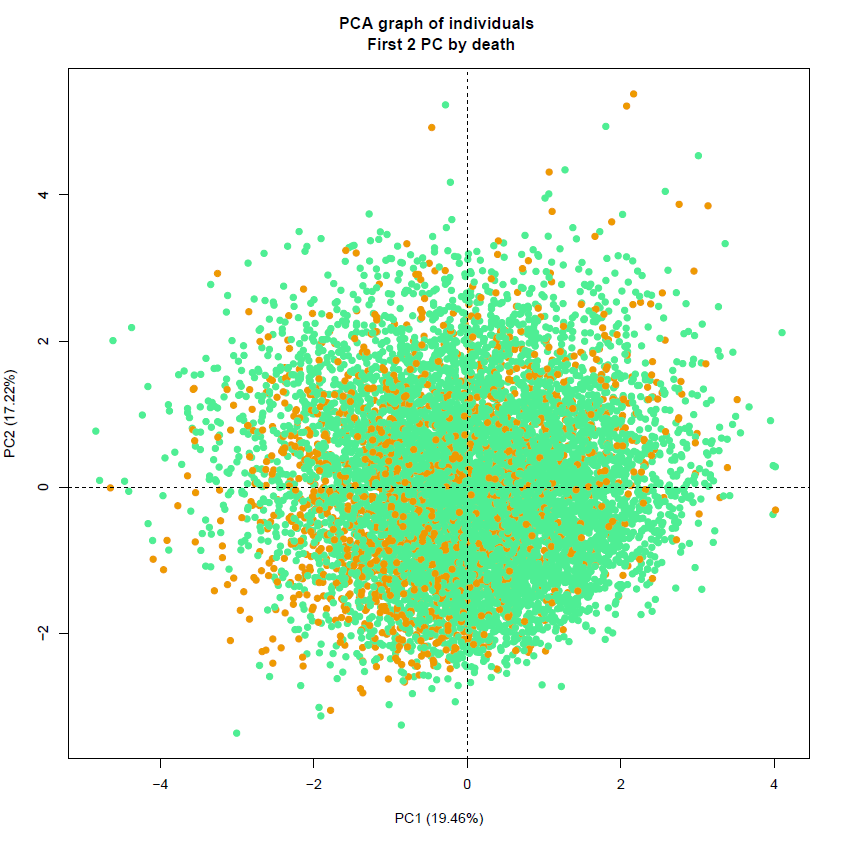
\includegraphics{../figure_output/pca_death.png}
\caption{First two PCs based on the sample covariance all population}
\end{figure}

In Figure 26, we plot the first two principal components considering the
entire population. Immediately, we observe that there is no clear
clustering of the data within the first two principal components. We
have broken out the data by survival (green) and death (orange), but we
see no clear linear relationship here either. Effectively, the full data
set appears uniformly distributed about the origin. We remark that the
density of orange points is more pronounced on the left quadrants,
implying the proportion of death outcomes is somewhat greater for
negative values of the first principal component, but uniformly
distributed in the second.

We note that the first two principal components represent approximately
40\% of the total variance explained in the model. This is less than
half the explained variance of the model and may seem less than ideal,
but as mentioned previously, our goal is to identify prominent clusters
more so than building an optimal alternate model through dimensionality
reduction. In Figure \ref{fig:pcaeigv}, we see that the captured
variance for the sequence of eigenvalues does not exhibit a clear drop
after the first few values. Instead, we see that the marginal explained
variance decreases at a near constant rate. In fact, we see the greatest
decrease in marginal explained variance after the second principal
component. Thus, we will focus our analysis on the first two PCs.

\begin{figure}
\centering
\includegraphics{Step1_Project_files/figure-latex/l1pc-1.pdf}
\caption{Loadings for the first and sencond PCs
individually\label{fig:l1pc}}
\end{figure}

Now, we consider the derivation of the first two principal components
using loading plots, shown in Figure \ref{fig:l1pc}. These plots
describe the weight of each variable on the respective principal
component loadings. Weights with greater distances from zero imply a
greater influence on the respective PC.

First Principal Component:

\begin{itemize}
\tightlist
\item
  We have variable sbp with a weight around +0.5 and hr, log\_cc, and
  log\_ncell with weights near -0.5, and log\_rr, log\_ndaysicu with
  smaller weights around -0.25.
\item
  Variables age and log\_injurytime have no weight on this PC.
\item
  Our biometrics contribute the most weight to this PC, with sbp, hr,
  log\_cc, and log\_ncell with the most prominent weights. This feature
  may describe the effect of general patient health at the time of the
  accident.
\item
  Some studies, such as
  \href{https://pubmed.ncbi.nlm.nih.gov/11896505/}{Banegas et all} and
  \href{https://www.ahajournals.org/doi/full/10.1161/hs0901.095395}{Kurl
  et all} suggest that Systolic blood pressure is a more frequent
  cardiovascular risk factor than other blood-related measures and can
  be used to detect future diseases, which may explain its prominence.
\end{itemize}

Second Principal Component:

\begin{itemize}
\tightlist
\item
  We have log\_ndaysicu and log\_injurytime with weights near +0.5, and
  age, sbp, and log\_ncell with weights around +0.25, and hr, log\_rr
  with weights near -0.25.
\item
  Variable log\_cc has a weight of zero.
\item
  We notice the contribution of age and log\_injurytime to the second
  PC, while not present in the first.
\item
  The variables log\_ndaysicu and log\_injurytime contribute the most
  weight to the second PC, so this feature describes the temporal
  context of the injury and recovery period.
\item
  This may suggest that prompt medical attention increases chances for
  survival.
\end{itemize}

We continue our analysis of the PC loadings with Figure \ref{fig:l3pc},
which provides a 2D loading plot.

\begin{figure}
\centering
\includegraphics{Step1_Project_files/figure-latex/l3pc-1.pdf}
\caption{Loadings for the first two PC\label{fig:l3pc}}
\end{figure}

We immediately note the most prominent variables: sbp, log\_ndaysicu,
log\_ncell, and hr. Moreover, we may consider the geometry between the
two PC axes. For this plot, the angles between the vectors provide
information on how characteristics are correlated. Small angles imply
positive correlations, large angles near 180° imply negative
correlation, while orthogonality implies unlikely correlation.

We notice a possible negative correlation between sbp and the other
biometrics log\_rr, log\_cc, and hr. In order to make conclusions, We
consider possible explanations for this behavior based on medical
studies:

\begin{enumerate}
\def\labelenumi{\arabic{enumi}.}
\item
  \href{https://clinicalhypertension.biomedcentral.com/articles/10.1186/s40885-017-0071-3}{Herakova
  et all} report the relationship between the increase of blood pressure
  during exhalation and the decrease during inhalation. Moreover, the
  paper mentions that in general deep breathing could reduce blood
  pressure.
\item
  \href{https://www.health.harvard.edu/heart-health/does-heart-rate-affect-blood-pressure}{Harvard
  Heart Letter} reports that an \emph{isolated increase in blood
  pressure can drop the heart rate a little}. As a result, after a
  patient's trauma, the increase in \emph{sbp} is followed by a decrease
  in heart rate, providing a possible explanation for the inverse
  relationship.
\end{enumerate}

\begin{itemize}
\item
  We notice a strong positive correlation between \emph{log\_injurytime}
  and \emph{age}, which we discussed in our previous sections. Greater
  age tends to be correlated with lower survival rates and longer
  treatment times.
\item
  There is no relation between the \emph{ndaysicu} with the biometrical
  measures as \emph{sbp} and \emph{hr}. It makes sense because this is a
  variable more related to medical attention. On the other hand
  \emph{ndaysicu} is more related to the variables \emph{ncell},
  \emph{injurytime}, and \emph{age}. This implies a strong association
  between our individual characteristics and the medical attention
  prescribed.
\end{itemize}

In figure 29, we see a very similar visualization as in Figure
\ref{fig:l3pc}, but with the observations included. Again, we notice a
lack of clustering, but we have an understanding of the relationships of
our characteristics.

\begin{figure}
\centering
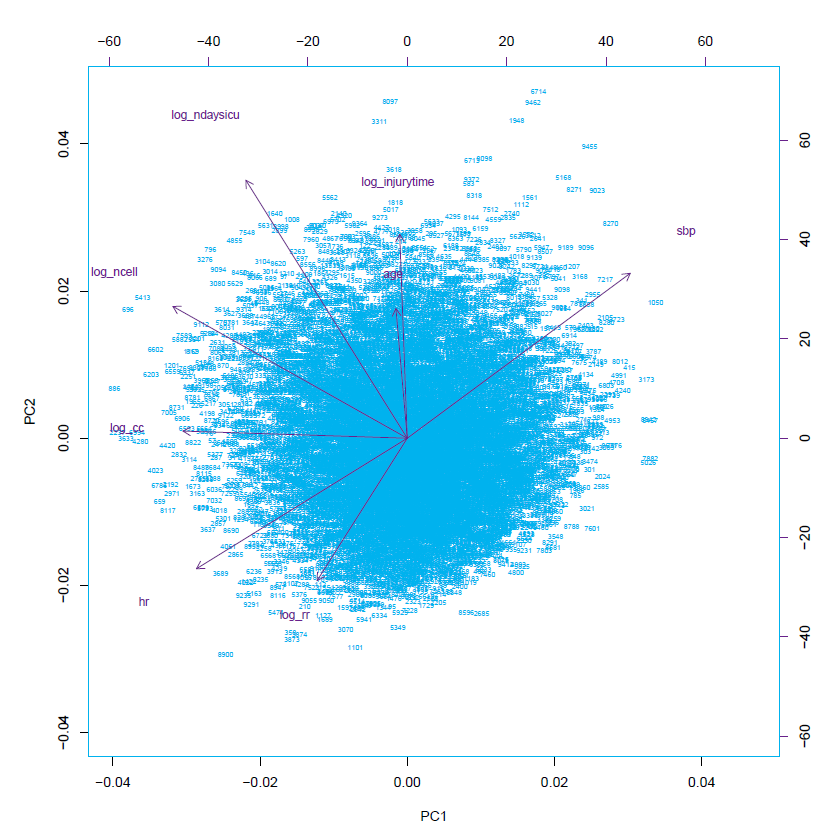
\includegraphics{../figure_output/pca_biplot.png}
\caption{PC Scores and PC loading all population}
\end{figure}

\newpage

Figure \ref{fig:pcaeigv} shows the explained variance of each
eigenvalue. As previously discussed, the first two PCs represent
approximately 40\% of the explained variance, but failed to reveal any
noticeable clusters. We see that the first four principal components
explain approximately 63\% of the model, this may provide more promising
groupings.

We must note that the shape of this plot alerts us that our data may not
be optimal to a standard PCA analysis. An ideal curve should be steep,
with the majority of the variance concentrated in the first few PCs,
then flatten out. Our curve, as discussed previously, decreases at a
steady rate with a heavy right tail. Even the first four PCs only
represent 63\% of the variance, which is less than optimal. The method
also failed to reveal any significant clusters. As a result, PCA may not
be the most appropriate dimensionality reduction technique for our data.

\begin{figure}
\centering
\includegraphics{Step1_Project_files/figure-latex/pcaeigv-1.pdf}
\caption{Eigenvalues of the sample correlation
matrix\label{fig:pcaeigv}}
\end{figure}

The matrix scatterplot in figure 31 reflects the relations in the first
four principal components. Here too, we do not appreciate a clear
distinction between the groups (death and survival). Nor do we see
linear relationships between the populations or a specific group. This
provides further justification for our initial decision of considering
only the first two PCs, since the subsequent two provide no further
insight into possible clusters.

\begin{figure}
\centering
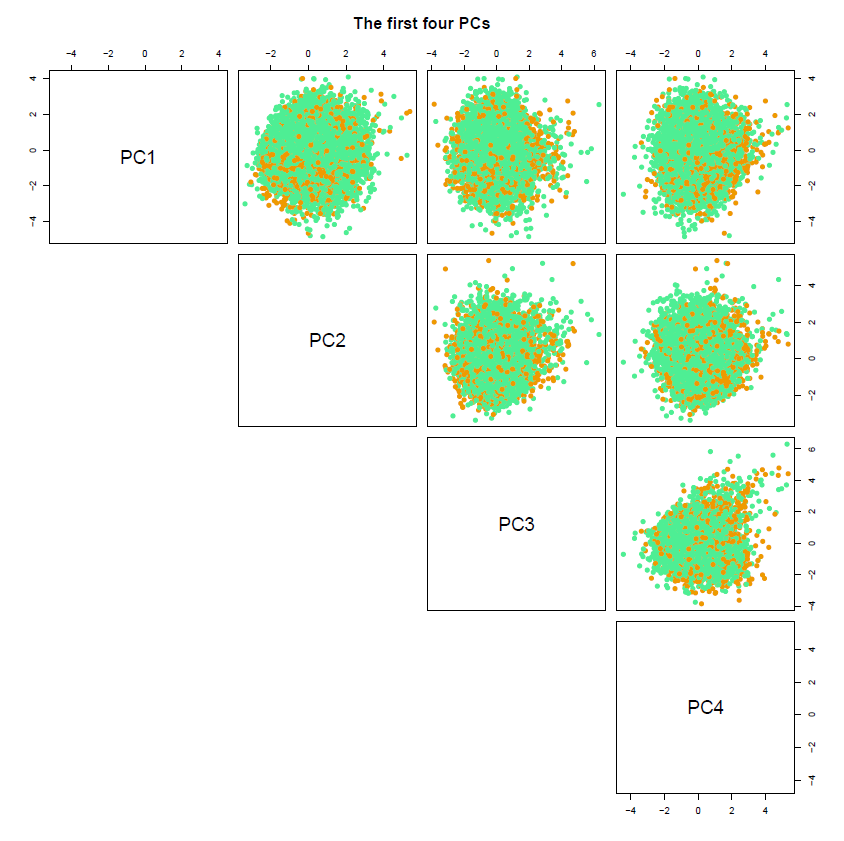
\includegraphics{../figure_output/pca_4pc2.png}
\caption{PC Scores and PC loading all population}
\end{figure}

Finally, figure \ref{fig:corrpc} explains the correlation between the
variables and the principal components. This information is very similar
to what we deduced graphically from the PC loadings plots. In the case
of the first principal components, in magnitude, the biometrical
measures and medical attention variables are more related to this
component. In the case of the second principal component, the individual
factors such as age and injury time acquire more relevance in the
analysis.

We see that for the third and fourth PC's, \emph{age} and \emph{log\_rr}
represent the most prominent weights. In the case of PC4, the positive
correlation between age and death becomes clear with the right skewed
distribution of the orange points in the matrix scatterplot in figure
31.

\begin{figure}
\centering
\includegraphics{Step1_Project_files/figure-latex/corrpc-1.pdf}
\caption{Correlation between dataset and all PC\label{fig:corrpc}}
\end{figure}

\newpage

\hypertarget{pca-by-category}{%
\subsection{PCA by Category}\label{pca-by-category}}

To further our analysis, we break out our data by survival outcome and
develop the Principal component analysis for death (1825 individuals)
and survival (7672 individuals) groups. In this case, we add the sex of
the patients where females are the blue points and males are gray.

Similar to Figure 26, figure 33 shows there is no linear relation
between the populations and the sex subgroups. Also, both principal
components explain approximately 35\% of the variance for each subgroup.
This is similar to the PCA for all the population.

\begin{figure}
\centering
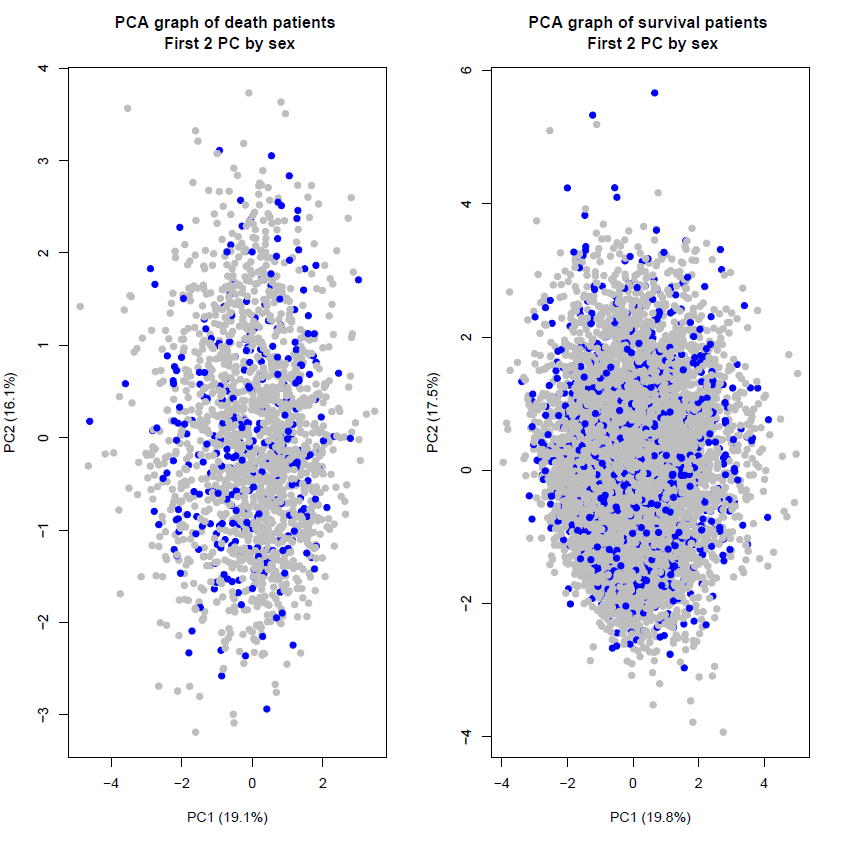
\includegraphics{../figure_output/pca_groups.png}
\caption{PC Scores and PC loading all population}
\end{figure}

In the case of the loadings for the first principal component (figure
\ref{fig:l1pcgrp}) for the death population, the largest positive values
are associated with \emph{hr} and \emph{cc}.

For the survival population, the first PC is greatly weighted by the
variables associated with medical attention such as \emph{ndaysicu} and
\emph{ncell}. As a result, we can observe the effect of receiving
medical attention as a crucial factor for survival in case of accident
or trauma. The variable sbp also has a significant negative weight.

The variable \emph{injurytime} has no significant effect on the survival
of the patients, but does weigh prominently in the first PC of the death
group. We also notice that sbp has considerable weight for both groups.

When we compare this results with the result of the PCA for all the
population, we appreciate that the effect of the medical attention is
more relevant for the second principal component than for the first one.

\begin{figure}
\centering
\includegraphics{Step1_Project_files/figure-latex/l1pcgrp-1.pdf}
\caption{Loadings for the first PC by death and survival
patients\label{fig:l1pcgrp}}
\end{figure}

Then, for the loading of the second principal component (figure
\ref{fig:l2pcgrp}), in the case of the death population, the effect of
the medical attention is reflected with the fact that \emph{ndaysicu}
and \emph{ncell} have the largest positive values. On the other hand,
for the loadings of the second principal component for survival
population, we can see how these variables are again relevant, but also
are important the variables of \emph{injurytime} and \emph{sbp}. So, the
second principal component for survival population reflects the effect
of receiving faster medical help. This effect was also reflected in the
second principal component for the general population.

\begin{figure}
\centering
\includegraphics{Step1_Project_files/figure-latex/l2pcgrp-1.pdf}
\caption{Loadings for the second PC by death and survival
patients\label{fig:l2pcgrp}}
\end{figure}

\newpage

Figure \ref{fig:l3pcgrp} shows the PCA graph for loading and scores. For
the Death patients, we notice the strong weight and positive correlation
of \emph{log\_ndaysicu} and \emph{log\_injurytime}. A second prominent
group of variables is \emph{log\_ncell}, \emph{hr}, and \emph{log\_cc}
which are strongly correlated together, but seemingly uncorrelated with
the other group and negatively correlated with sbp. This aligns with our
earlier observation, that elevated Systolic Blood Pressure may decrease
heart rates.

\begin{figure}
\centering
\includegraphics{Step1_Project_files/figure-latex/l3pcgrp-1.pdf}
\caption{Loadings for the first two PC by death and survival
patients\label{fig:l3pcgrp}}
\end{figure}

For Survival patients, right panel of figure \ref{fig:l3pcgrp}, we
notice slightly different correlation patterns. For example,
\emph{log\_ndaysicu} and \emph{log\_ncell} are positively correlated and
significant for both PCs. For patients who survive, the duration and
intensity of treatment are positively correlated. Meanwhile, for
patients who do not survive, we see a correlation between the duration
of treatment and the time of injury, independent of the intensity of
treatment. For both groups, the intensity of treatment and time of
injury are not correlated.

A variable that we would benefit from here is a measure of the severity
of the trauma, which would provide a more nuanced understanding of these
relationships. It is likely that a majority of those who survive
suffered less intense wounds than those who died. This would explain why
duration and intensity of treatment are correlated for survival
patients, since this would most likely be indicative of progressively
severe wounds. Meanwhile, for patients who do not survive, duration and
intensity of treatment are not correlated, which may be because these
patients generally suffered the most severe wounds and had low chances
of survival. Thus, the speed at which they were able to begin treatment
only bought them time, regardless of the treatment. If we had more
information on the type and severity of the wounds, we would be able to
test this hypothesis.

\begin{figure}
\centering
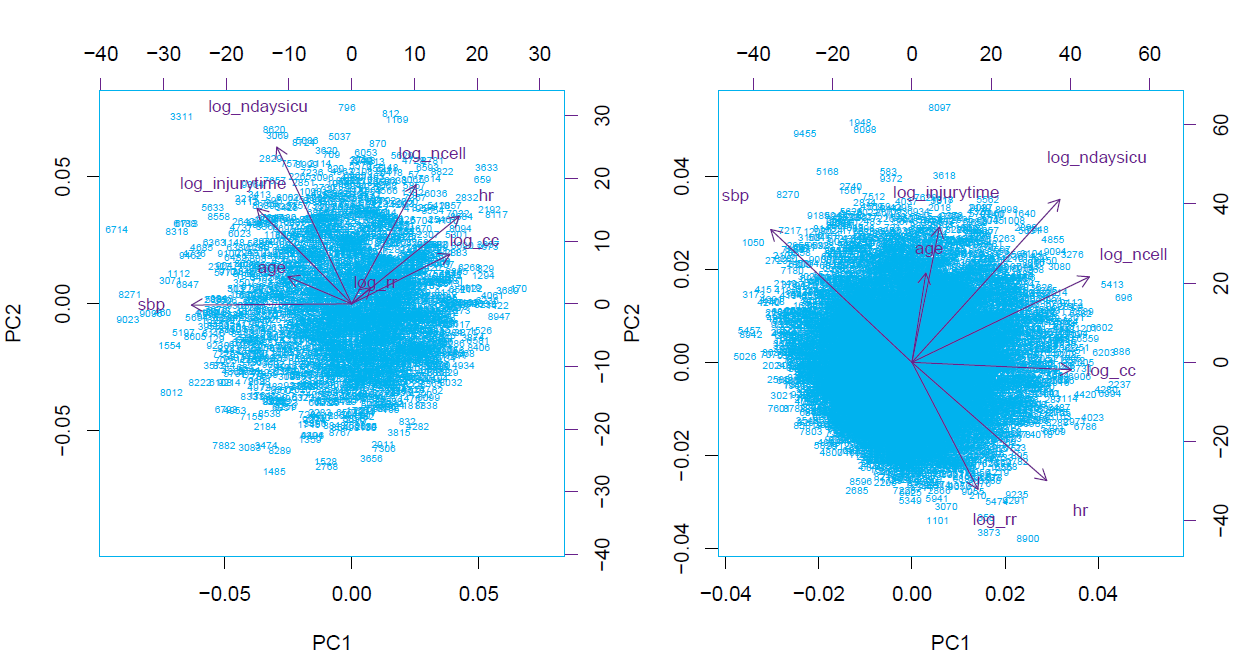
\includegraphics{../figure_output/pca_group_biplot}
\caption{PC Scores and PC loading all population for death and survival
patiens}
\end{figure}

We have our PC Score plots with the observations mapped in figure 37.
This is somewhat redundant and confirms our observations that there are
no clear clusters and reiterates the correlations we discussed
previously.

Finally, figures \ref{fig:pcaeigvgr1} and \ref{fig:pcaeigvgr2} provide
us with the variance plots for the eigenvalues of the two groups.
Similarly to the full population, we see that we have less than ideal
reorganizations of the data using PCA on these two groups. The shape of
the curves is almost linear, decreasing at a near-constant rate. This is
not an ideal distribution of variance across principal components, where
we would like a greater concentration at the top of the tail. We may
want to consider alternative approaches to dimensionality reduction for
this data.

\begin{figure}
\centering
\includegraphics{Step1_Project_files/figure-latex/pcaeigvgr1-1.pdf}
\caption{Eigenvalues of the sample correlation matrix for death
patients\label{fig:pcaeigvgr1}}
\end{figure}

\begin{figure}
\centering
\includegraphics{Step1_Project_files/figure-latex/pcaeigvgr2-1.pdf}
\caption{Eigenvalues of the sample correlation matrix for survival
patients\label{fig:pcaeigvgr2}}
\end{figure}

\newpage

\hypertarget{conclusions}{%
\subsection{Conclusions}\label{conclusions}}

The purpose of this study was to extract insights from our data using
Principal Component Analysis. We selected a large data set and selected
a subset of categorical and continuous variables for our analysis. Since
we manually removed a number of variables, eliminating any pressing need
for dimensionality reduction, our primary use for PCA was to identify
any groups in the data and understand patterns regarding survival
outcomes and treatment.

Our preliminary treatment of the data involved standardizing variables
with significant skew using log transformations. We assessed the
behavior of our continuous variables across different categories,
finding strong patterns in age, injury time, and central capillary
refill time in terms of survival outcomes. Using sample correlation
matrices, we noticed recorded our strongest positive correlation between
log\_ncell and log\_ndaysicu, relating the duration and intensity of
treatments. We also noted negative correlations between Systolic Blood
Pressure and other biometrics like Heart Rate and Respiratory Rate,
which may be explained by the physiological effects of blood pressure on
respiration.

Our application of Principal Component Analysis revealed no clusters in
our data, even with breakdowns by sex and survival. However, we were
able to more precisely assess the relationship between our variables and
gain valuable insight into possible indicators of survival as well as
multivariate patterns. We notice that for the general population, the
first principal component is constructed mainly with the biometrics,
while the second PC is weighted more by treatment times. This provides
evidence for the importance of general biometric indicators, like blood
pressure and respiratory rates, to understand the status of a patient.

We must note the sub-optimal distribution of variance across the
principal components in the eigenvalue plots, which indicates that this
method may not be appropriate for our data as is. Effectively, the
behavior of our observations cannot be fully explained by a minimal
number of feature vectors.

Through a categorical breakdown of PCA, we were able to assess
differences in correlations between injury time, duration of
hospitalization, and the intensity of treatment between patients who
survive and those who do not. For survival patients, the duration and
intensity of treatment are positively correlated, while patients who
died show a positive correlation between the duration of treatment and
the time of injury. In both groups, time of injury and intensity of
treatment are not correlated.

This small divergence across groups may have alerted us to a broader and
critical issue: existing patterns in our data are not adequately
expressed by the variables we chose in our initial selection. It is our
suspicion that below our indicators for survival, there runs a current
of behavior related to the \emph{intensity of injury} that wields
considerable influence on survival outcomes, the efficacy of treatment,
and the biometrics. Unexpressed and dictatorial in its causality, this
subliminal information may be the primary agent of sabotage in the
restructuring of variance under the principal components, since the most
profound agent of behavior remains hidden from us. This is easily
grasped: the type and severity of treatment are fundamental in
determining treatment options and are strongly correlated with the
likelihood of survival.

Unfortunately, none of our selected variables provide even the most
tangential information regarding the type and severity of the injury.
Thus, this crucial information cannot even be inferred. However, the
original data set did include such information. As such, we recommend
that any further work on this analysis include a reconsideration of the
selection of variables, where more information regarding the type and
severity of injury be included in the data set.

\hypertarget{references}{%
\subsection{References}\label{references}}

\begin{enumerate}
\def\labelenumi{\arabic{enumi}.}
\item
  Banegas JR, de la Cruz JJ, Rodriguez-Artalejo F, Graciani A,
  Guallar-Castillon P, Herruzo R. Systolic vs diastolic blood pressure:
  community burden and impact on blood pressure staging. J Hum
  Hypertens. 2002 Mar;16(3):163-7. doi: 10.1038/sj.jhh.1001310. PMID:
  11896505.
\item
  S. Kurl, J.A. Laukkanen, R. Rauramaa, T.A. Lakka, J. Sivenius, and
  J.T. Salonen. Systolic Blood Pressure Response to Exercise Stress Test
  and Risk of Stroke. Sep 2001
  \url{https://doi.org/10.1161/hs0901.095395Stroke}. 2001;32:2036--2041
\item
  Ratner, B. The correlation coefficient: Its values range between
  \(+1/-1\), or do they? J Target Meas Anal Mark 17, \(139-142\) (2009).
  \url{https://doi.org/10.1057/jt.2009.5}
\end{enumerate}

\end{document}
